\chapter{Algorithm Design}\label{chapAlogrithmDesign}

The approach is based on a \gls{GeneticProgramming}, as decided in chapter \ref{chapAlgorithmicApproach}. Section \ref{secAlgorithmOverview} describes the algorithm. In section \ref{secMutationAndFitnessFunctionDesignProcess} details about the design method of the core entities are provided. Those are \glspl{Mutation} and \glspl{FitnessFunction}. Section \ref{secPatternAndMutations} explains the \glspl{Mutation} used in the algorithm with its associated pattern. The further sections describe the alternative strategies within fitness evaluation (section \ref{secFitnessFunctions}), selection and replacement (section \ref{secSelectionReplacementStrategies}) and mutation selection (section \ref{secMutationSelectionStrategies}).

\section{Algorithm Overview}
\label{secAlgorithmOverview}

The used \gls{EvolutionaryAlgorithm} has been derived from \cite{Ashlock2004} and is shown in its modified version in figure \ref{figEvolutionaryAlgorithm}. It splits up into six phases, distributed among four components, which are described after the general design decisions in the following. 

\begin{figure}[htb]
	\centering
	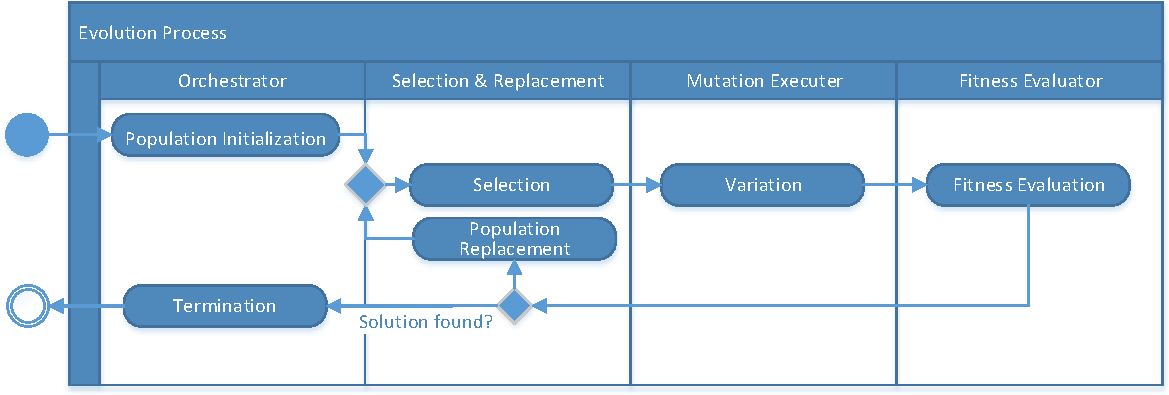
\includegraphics[scale=0.75]{Images/AlgorithmEA.pdf} 
	\caption{Evolutionary Algorithm (\cite{Ashlock2004})}
	\label{figEvolutionaryAlgorithm}
\end{figure}

As explained in section \ref{secTransformationComplexity}, the problem of generating \glspl{ModelToModelTransformation} is difficult to tackle. Since an \gls{EvolutionaryAlgorithm} itself is a general construct, it does not provide guidance for this particular issue. Therefore, the complexity is captured by a tailored method, which uses complex \glspl{GeneticOperator} that create \glspl{ModelToModelTransformation} based on design patterns.

The common approach in the field of \glspl{EvolutionaryAlgorithm} is to handle the complexity with the \gls{FitnessFunction}. Using it for this problem would result in generic \glspl{GeneticOperator} that are only based on the information provided by the \gls{TransformationLanguage} and \gls{MetaObjectFacility} definition. Hence, the created \glspl{ModelToModelTransformation} are not comprehensible and would cause only in very rare cases a measurable fitness change. In the case the majority of the \gls{GeneticOperator} modifications does not result in a fitness change, the algorithm has no guidance. This is a random search. Thus, more information has to be considered in the \gls{FitnessFunction}. In addition to the output of the \gls{ModelToModelTransformation}, also the transformation itself must be analyzed. This analysis is a reverse engineering of the \glspl{ModelToModelTransformation}, which is not part of the chosen approach (see \ref{chapAlgorithmicApproach}). Hence, such generic \glspl{GeneticOperator} are not used. Instead, they are based on design pattern and not directly on the \gls{TransformationLanguage}.

Figure \ref{figEvolutionaryAlgorithm} shows the algorithm, with four of the six phases placed into two components. Initialization and Termination are within the Orchestrator, since those are closely related by providing the general frame of the execution. Furthermore, the Selection and Population Replacement are in a single component. They depend on interleaved strategies rendering selection and replacement tightly coupled.

The following paragraphs describe each phase of the algorithm and highlight the entities which have alternatives. Those are visualized in the figures with a dark blue shape and an underscore. They have an impact on the performance and quality of the algorithm. In chapter \ref{chapEvaluation} the optimum values within the scenarios are determined and explained.

\begin{figure}[htb]
	\centering
	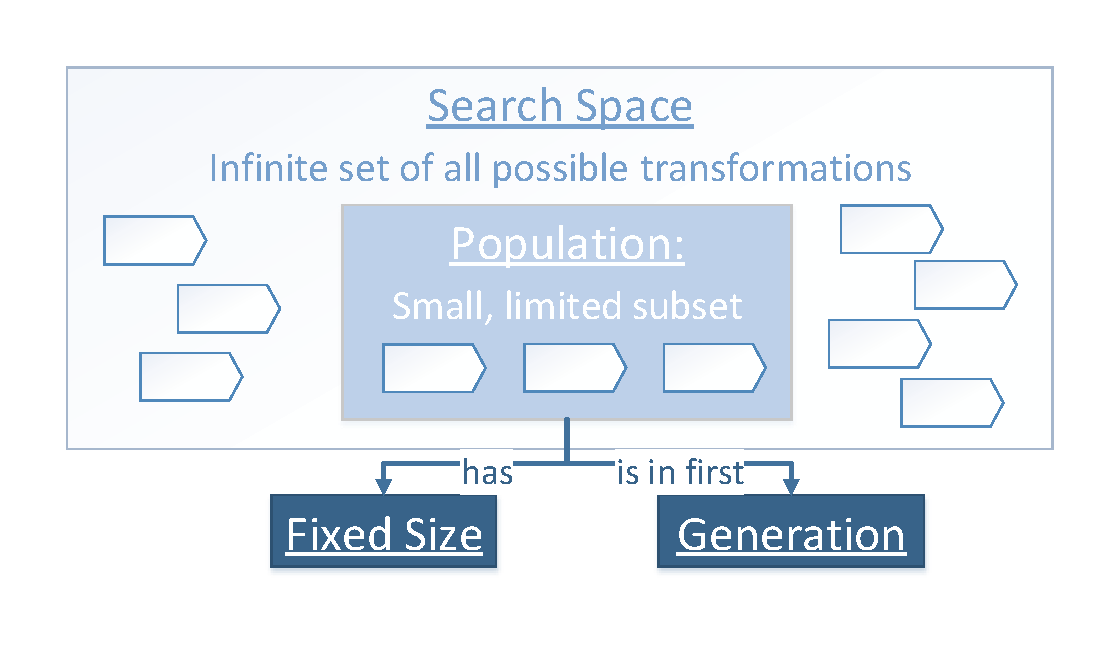
\includegraphics[scale=0.5]{Images/Algorithm_01_PopulationInitialization.pdf} 
	\caption{Population Initialization: The initial \gls{Population} is a small subset of the \gls{SearchSpace} with a fixed size and represents the first generation. Each \gls{Individual} inside is an empty \gls{ModelToModelTransformation}.}
	\label{figAlgorithm_01_PopulationInitialization}
\end{figure}

\textbf{1) Population Initialization}: In the first phase the initial \gls{Population} is created. It represents the first generation with a fixed number of \glspl{Individual}, which are \glspl{ModelToModelTransformation} (see figure \ref{figAlgorithm_01_PopulationInitialization}). Ideally, those are spread across the \gls{SearchSpace}, but as it is infinite this is not feasible. An approximation is to limit the \gls{SearchSpace}, e.g. by a maximum graph size, and by defining a method to spread. Since the approach is pattern based, such a method must be based on those. Applying patterns is equivalent to the application of \glspl{GeneticOperator} within the next execution phases. Hence, the algorithm initializes the \glspl{Individual} with empty \glspl{ModelToModelTransformation}. The bootstrap challenge, which is the issue of not being able to find a proper initial \gls{Population}, is handled by the Mutation Selection Strategies (see section \ref{secMutationSelectionStrategies}). Furthermore, in this phase the size of the \gls{Population} is defined, which will be kept during the execution and therefore is an important factor for the algorithm performance.

\begin{figure}[htb]
	\centering
	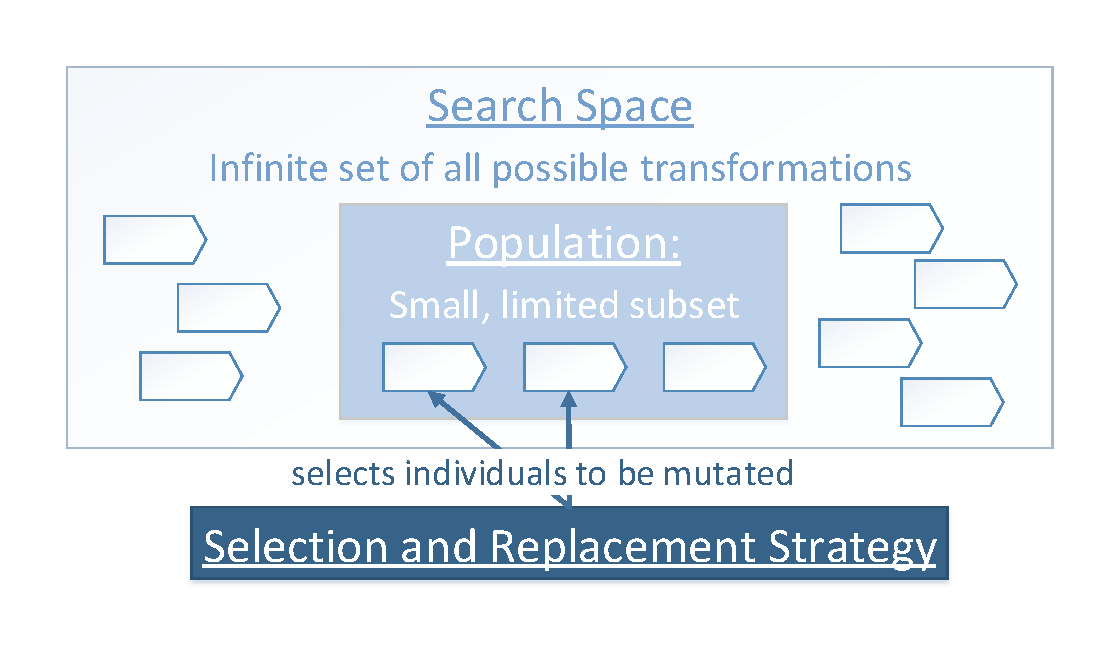
\includegraphics[scale=0.5, trim=0cm 1cm 0cm 1cm, clip=true]{Images/Algorithm_02_Selection.pdf} 
	\caption{Selection: The \gls{SelectionStrategy}, which is part of the Selection and Replacement Strategy, determines \glspl{Individual} in the \gls{Population} that are variated in the next phase.}
	\label{figAlgorithm_02_Selection}
\end{figure}

\textbf{2) Selection}: This phase is the start of the evolution, which requires at first the selection of \glspl{Individual} for the subsequent variation (see figure \ref{figAlgorithm_02_Selection}). The selection alternatives are described in section \ref{secSelectionReplacementStrategies}.

\begin{figure}[htb]
	\centering
	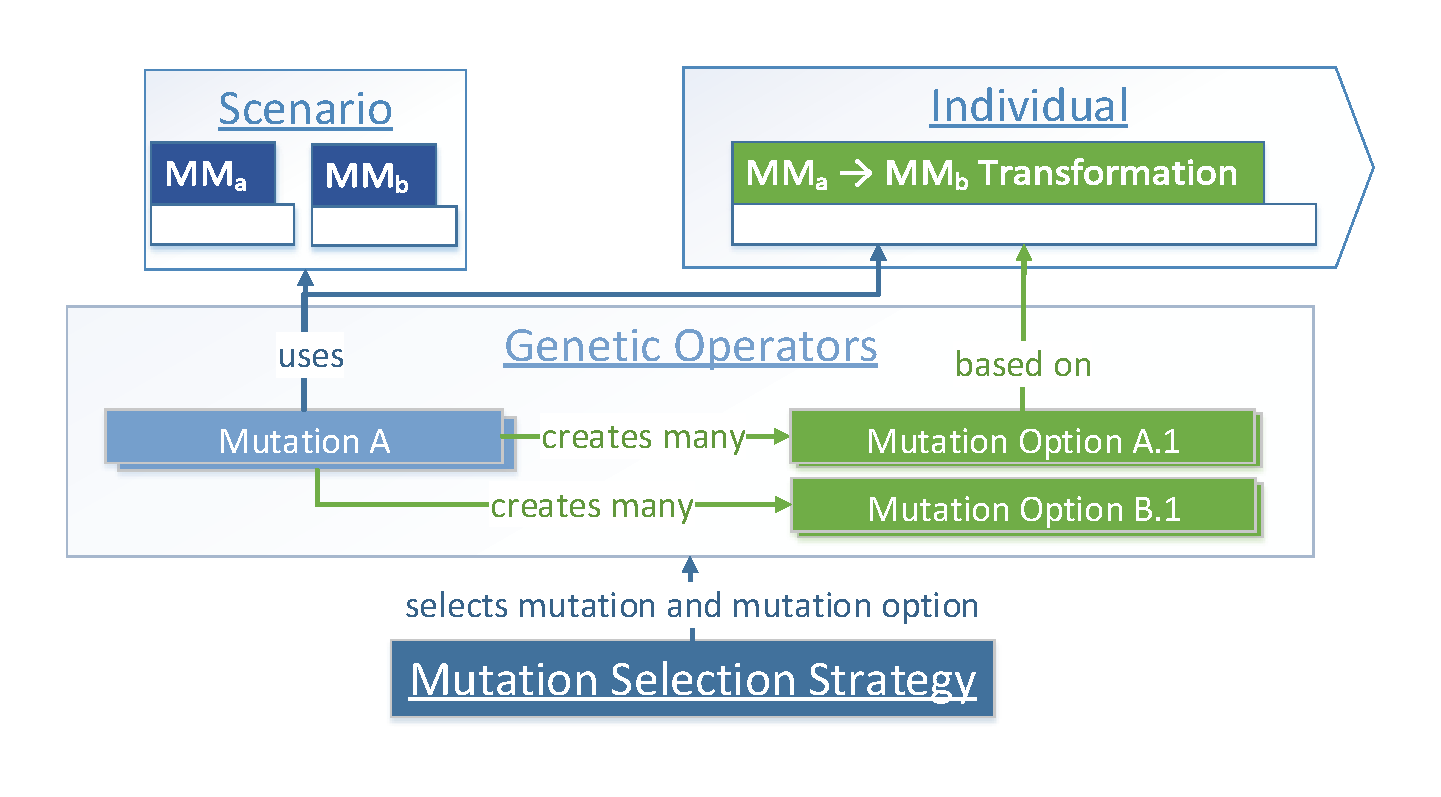
\includegraphics[scale=0.5, trim=0cm 1cm 0cm 1cm, clip=true]{Images/Algorithm_03_Variation_A.pdf} 
	\caption{Variation Step 1: The \glspl{GeneticOperator}, which are all \glspl{Mutation}, use the scenario \glspl{MetaModel} MM$_a$, MM$_b$ and the \gls{ModelToModelTransformation} in the \gls{Individual} to create the context specific mutation options. The Mutation Selection Strategy then selects a \gls{Mutation} and one of the options.}
	\label{figAlgorithm_03_Variation_A}
\end{figure}

\begin{figure}[htb]
	\centering
	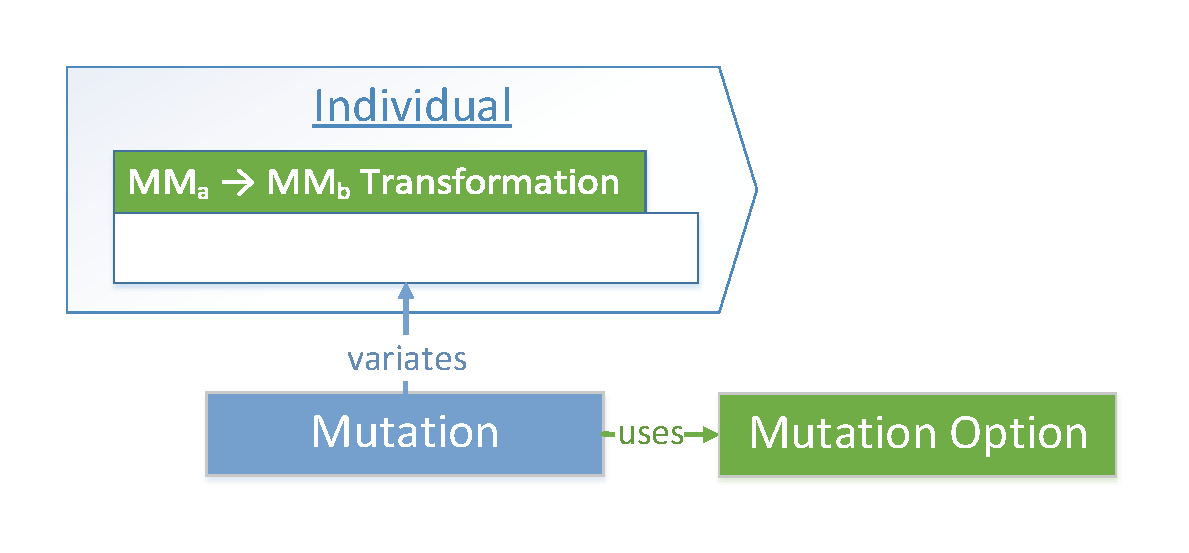
\includegraphics[scale=0.5, trim=0cm 1cm 0cm 1cm, clip=true]{Images/Algorithm_03_Variation_B.pdf} 
	\caption{Variation Step 2: The \gls{Mutation} variates the \gls{ModelToModelTransformation} in the \gls{Individual} using the selected option.}
	\label{figAlgorithm_03_Variation_B}
\end{figure}

\textbf{3) Variation}: As explained in the general design decisions previously in this section, the complexity is tackled by \glspl{GeneticOperator}. They are based on the transformation pattern described in chapter \ref{chapM2MScenarios}. The consequence is that there are multiple operators and each operator has several options in a specific \gls{ModelToModelTransformation}. For example the creation of a \gls{TransformationRule} is an operator. When applied to a transformation of the scenario, where already several rules exist, only the not yet existing ones are such an option. Hence, an option is an instance of a \gls{Mutation}. Furthermore, all operators are \glspl{Mutation} without \glspl{Crossover}, since those are mandatory and were sufficient to solve the scenarios (see chapter \ref{chapEvaluation}). Thus, the first step is to select a \gls{Mutation}, which is described in section \ref{secPatternAndMutations}, and an option using a Mutation Selection Strategy presented in section \ref{secMutationSelectionStrategies} (see figure \ref{figAlgorithm_03_Variation_A}).

The second step is the variation of the \gls{ModelToModelTransformation} with the selected \gls{Mutation} and option (see figure \ref{figAlgorithm_03_Variation_B}).

\begin{figure}[htb]
	\centering
	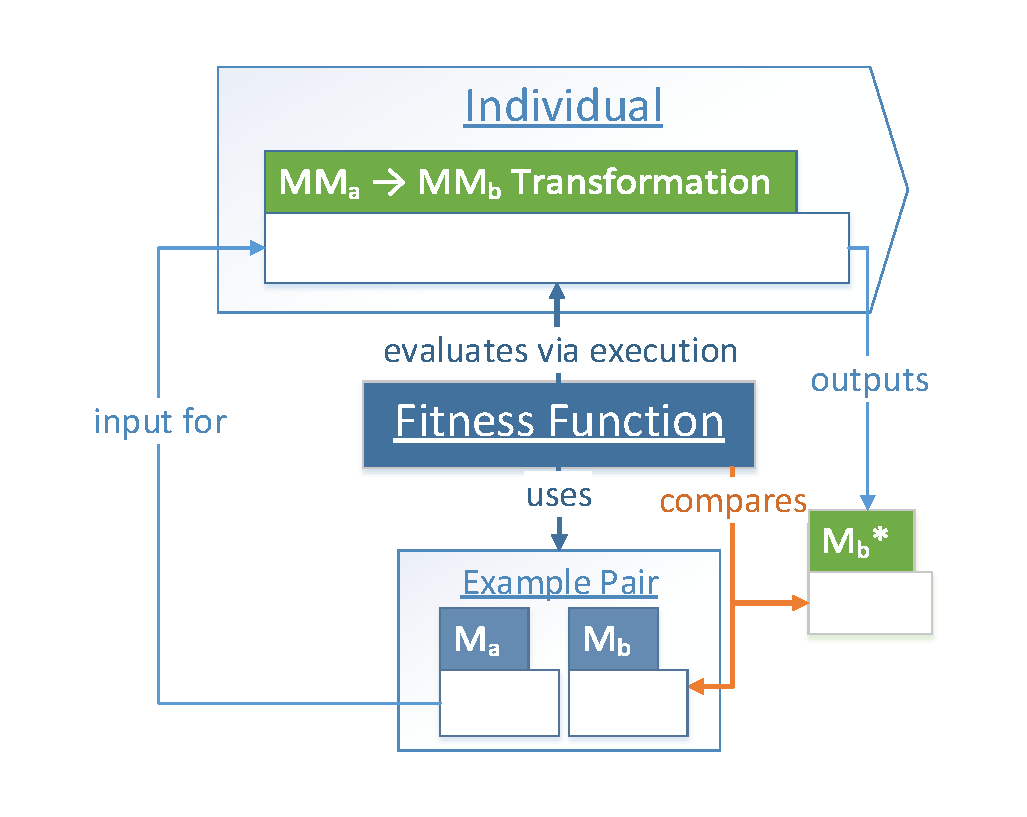
\includegraphics[scale=0.5, trim=0cm 1cm 0cm 1cm, clip=true]{Images/Algorithm_04_FitnessEvaluation.pdf} 
	\caption{Fitness Evaluation: The \gls{FitnessFunction} evaluates the \gls{ModelToModelTransformation} by executing it with the \gls{Model} M$_a$ of the example pair. The resulting \gls{Model} M$_b^*$ is the compared to the example M$_b$.}
	\label{figAlgorithm_04_FitnessEvaluation}
\end{figure}

\textbf{4) Fitness Evaluation}: All variated \glspl{Individual} require an update of the fitness, which is performed in this phase (see figure \ref{figAlgorithm_04_FitnessEvaluation}). The \gls{FitnessFunction} executes the \gls{ModelToModelTransformation} with the \gls{Model} M$_a$ of the example pair. The result M$_b^*$ of this execution is compared with the expected M$_b$ and the differences are then computed into a fitness value. There are several alternatives for the \gls{FitnessFunction} which are described in section \ref{secFitnessFunctions}.

\begin{figure}[htb]
	\centering
	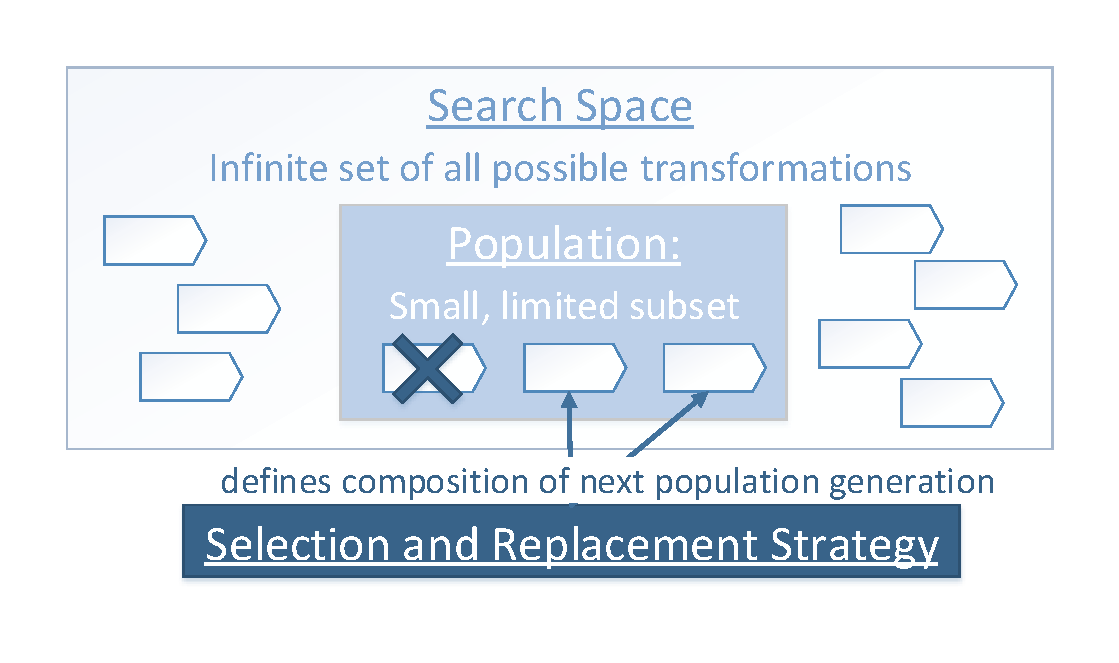
\includegraphics[scale=0.5, trim=0cm 1cm 0cm 1cm, clip=true]{Images/Algorithm_05_Replacement.pdf} 
	\caption{Population Replacement: The \gls{ReplacementStrategy} assembles the next generation of the \gls{Population}}
	\label{figAlgorithm_05_Replacement}
\end{figure}

\textbf{5) Population Replacement}: The last step of the evolutionary cycle is the assembly of the next generation of the \gls{Population} (see figure \ref{figAlgorithm_05_Replacement}). The \gls{ReplacementStrategy}, which is part of the Selection and Replacement Strategy, is applied, whereas the alternatives are described in sub-section \ref{secSelectionReplacementStrategies}.

\textbf{6) Termination}: The algorithm stops in case a transformation is found that produces exactly all the expected M$_b$ \glspl{Model}. Additionally, it stops when a maximum number of \glspl{Generation} is reached. From the solution or \gls{CandidateSolution} with the best fitness, all constructs which do not decrease the fitness are removed. This improves the readability of the \gls{ModelToModelTransformation}.

\newpage
\section{Transformation Pattern, Mutation and Fitness Function Design Method}
\label{secMutationAndFitnessFunctionDesignProcess}

The \gls{ModelToModelTransformation} complexity is primarily handled by the \glspl{Mutation} and also the closely related \gls{FitnessFunction}. Within this thesis, the created \glspl{Mutation} and the \gls{FitnessFunction} were targeted at the simple and complex scenario. Hence, they are not able to solve all possible scenarios. An extension of the algorithm is required for completely different scenarios. This section describes the extension design method in terms of the followed design process.

\begin{figure}[!ht]
	\centering
	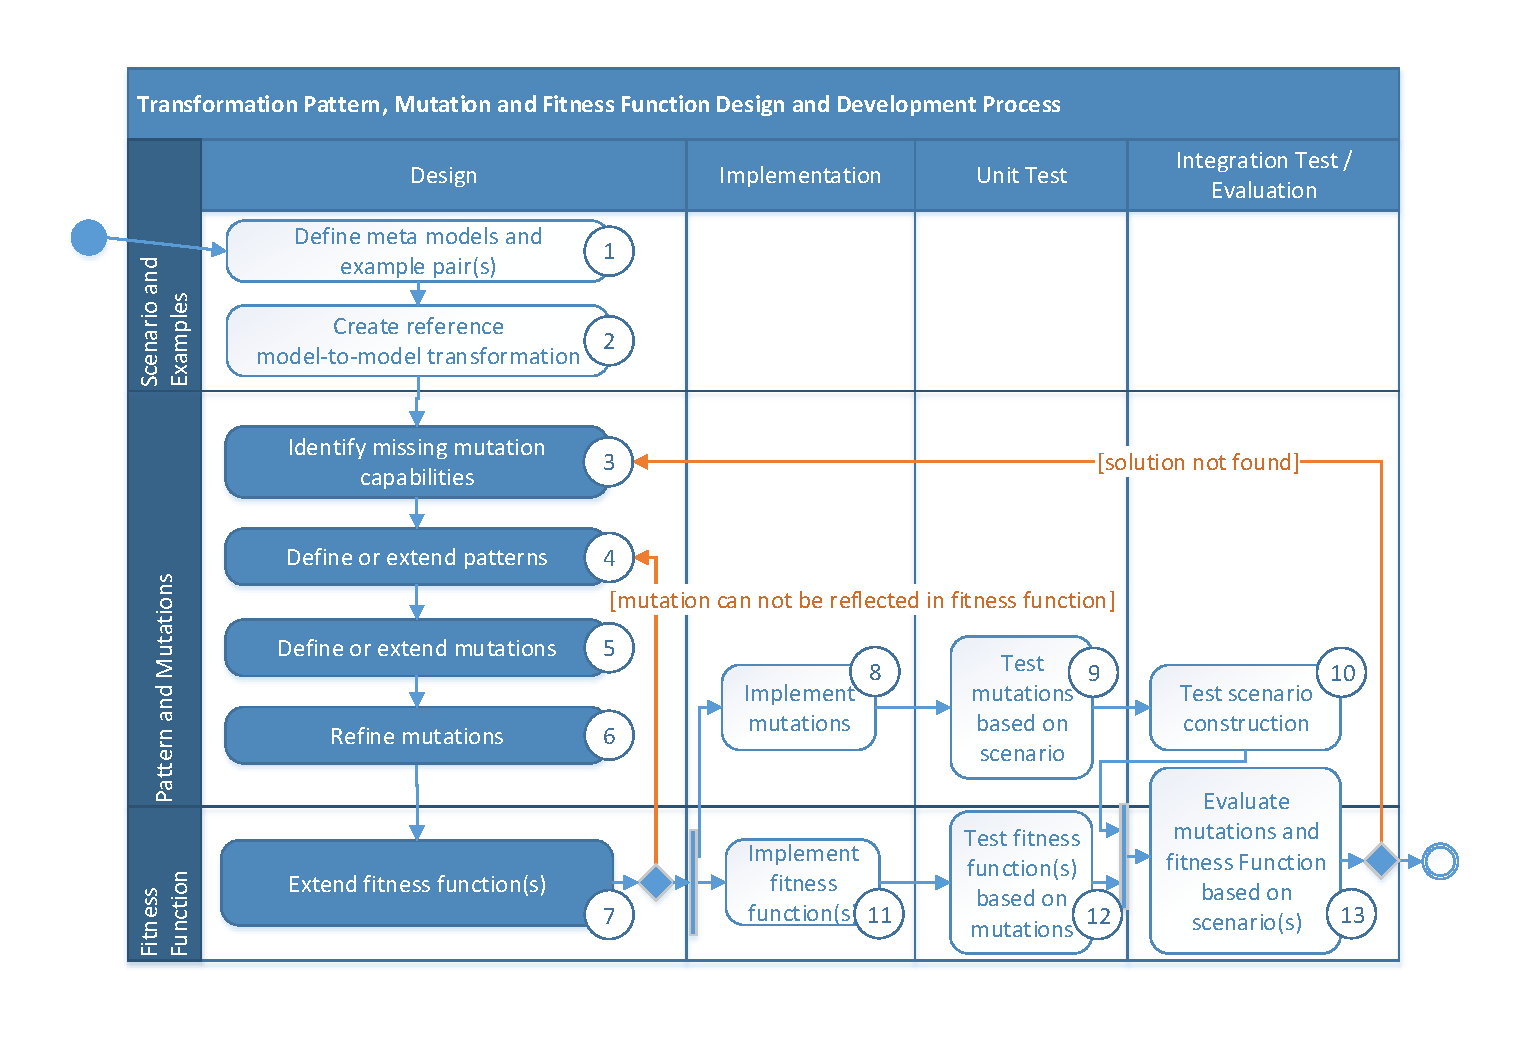
\includegraphics[scale=0.6, trim=0cm 1cm 0cm 1cm, clip=true]{Images/MutationAndFitnessFunctionDevelpomentProcess.pdf} 
	\caption{\Gls{Mutation} and \gls{FitnessFunction} design and development process}
	\label{figMutationAndFitnessFunctionDevelpomentProcess}
\end{figure}

Figure \ref{figMutationAndFitnessFunctionDevelpomentProcess} presents the design process in detail, based on the general process in section \ref{secDesignAndDevelopmentProcess}. The steps 3 to 7 are the main topics within this chapter and therefore highlighted in the overview. The details of step 1 and 2 are explained in chapter \ref{chapM2MScenarios}, while the description of step 8 to 13 is in chapter \ref{chapPrototypeDesign}. In the following paragraphs each step will be described with references to the simple and complex scenario.

\textbf{1) Define source and target \glspl{MetaModel} and example pair(s)}: Since there is no common definition of \glspl{ModelToModelTransformation}, the approach is based on representative scenarios which contain a source and target \gls{MetaModel}. Those are described in chapter \ref{chapM2MScenarios} including the design considerations.

\textbf{2) Create a reference \gls{ModelToModelTransformation}}: The \glspl{MetaModel} of the scenario can be transformed in infinite ways. However, for the desired approach the definition of a desired transformation is required (see figure \ref{figMutationAndFitnessFunctionDesignProcess-Step2}). This is the foundation for the identification of the necessary \glspl{Mutation}. Since the result produced by the algorithm is not always complete, the created transformations should be comprehensible by humans. Thus, the design goal is not a transformation which could be automatically created easily, but which is readable.

\begin{figure}[!ht]
	\centering
	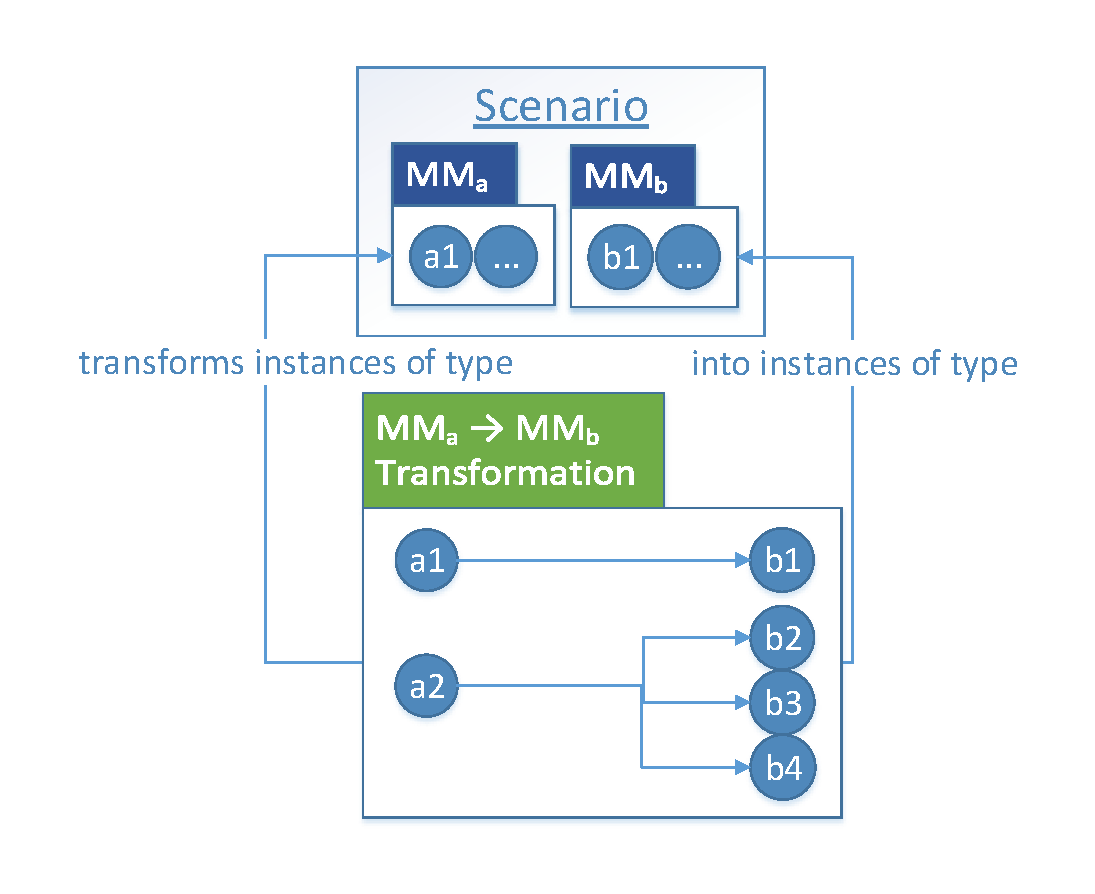
\includegraphics[scale=0.5, trim=0cm 1cm 0cm 1cm, clip=true]{Images/MutationAndFitnessFunctionDesignProcess-Step2.pdf} 
	\caption{\Gls{Mutation} and \gls{FitnessFunction} design and development process - Step 2: Create a reference \gls{ModelToModelTransformation}}
	\label{figMutationAndFitnessFunctionDesignProcess-Step2}
\end{figure}


\textbf{3) Identify missing \gls{Mutation} capabilities}: In the case the scenario is not solvable with the given \glspl{Mutation}, the \gls{ModelToModelTransformation} will be inspected and the missing aspects highlighted (see figure \ref{figMutationAndFitnessFunctionDesignProcess-Step3}). 

The following example starts after the algorithm supports the simple scenario. Listing \ref{lstETLFragementOfComplexExample} shows a small fragment of the complex scenario showing the one-to-many rule that creates for a single outgoing transitions of a complex state, multiple transitions each starting at one of the inner states. The rule contains a loop which iterates over those states, creates a transition and adds this transition to the result list. Since the simple example does not require any of the mentioned aspects, none of those are supported.

\begin{lstlisting}[language=ETL,caption={Fragment of Complex State Machine to Simple State Machine \gls{ModelToModelTransformation} in \gls{ConcreteSyntax} of \Gls{EpsilonTransformationLanguage}},label={lstETLFragementOfComplexExample}]
rule TransitionFromComplexStateToManyTransitions
	transform sourceTransition : Source!Transition
	to targetTransitions : Sequence(Target!Transition) {
	...
	for(sourceState in sourceTransition.Source.States) {
		var targetTransition = new Target!Transition;
		targetTransitions.add(targetTransition);
		...
	}
}
\end{lstlisting}

\begin{figure}[!ht]
	\centering
	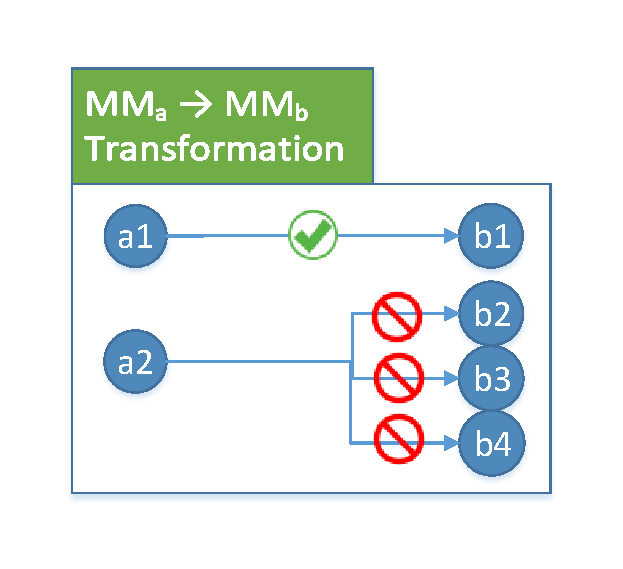
\includegraphics[scale=0.5, trim=0cm 1cm 0cm 1cm, clip=true]{Images/MutationAndFitnessFunctionDesignProcess-Step3.pdf} 
	\caption{\Gls{Mutation} and \gls{FitnessFunction} design and development process - step 3: Identify missing \gls{Mutation} capabilities}
	\label{figMutationAndFitnessFunctionDesignProcess-Step3}
\end{figure}


\textbf{4) Define or extend patterns}: The missing aspects, resulting from the previous step, have to be arranged into transformation patterns. Hence, the main task is to create or extend the set of transformation patterns (see figure \ref{figMutationAndFitnessFunctionDesignProcess-Step4}). The challenge is to create patterns that are not only tailored for the current scenario, but are also not too generic and thereby difficult to be captured by the \gls{FitnessFunction} in step 7. This is therefore the most important design step. 

Proceeding with the example presented in the previous step in listing \ref{lstETLFragementOfComplexExample}, this results in the following consideration: The whole loop structure is not yet included in any pattern. Thus, a pattern might create loop structures using some enumerable \gls{Property} from the ``sourceTransition" or ``targetTransition". This does not result in a different output M$_b^*$. Hence, this renders a measurement of any change in the output M$_b^*$ impossible in step 7. The pattern needs to be more coarse grained. In this case, the intention of the loop is to create multiple \glspl{Object} in the target \gls{Model} M$_b$ for a single one in the source. Using this information the pattern is ``One-to-Many" on M2 level with some restrictions regarding the enumerable resulting in the ``Many" \glspl{Object}. Figure \ref{figTransformationPattern_OneToManyObjectsOfSameType} shows this pattern, which is explained in section \ref{secPatternAndMutations}.

\begin{figure}[!ht]
	\centering
	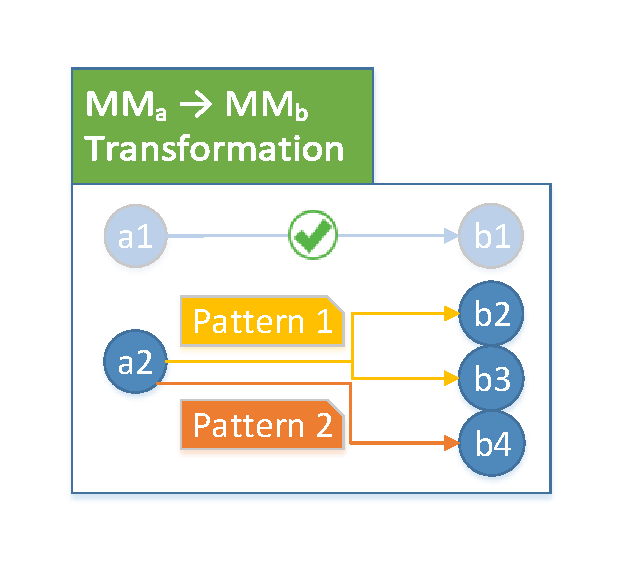
\includegraphics[scale=0.5, trim=0cm 1cm 0cm 1cm, clip=true]{Images/MutationAndFitnessFunctionDesignProcess-Step4.pdf} 
	\caption{\Gls{Mutation} and \gls{FitnessFunction} design and development process - step 4: Define or extend patterns}
	\label{figMutationAndFitnessFunctionDesignProcess-Step4}
\end{figure}


\begin{figure}[!ht]
	\centering
	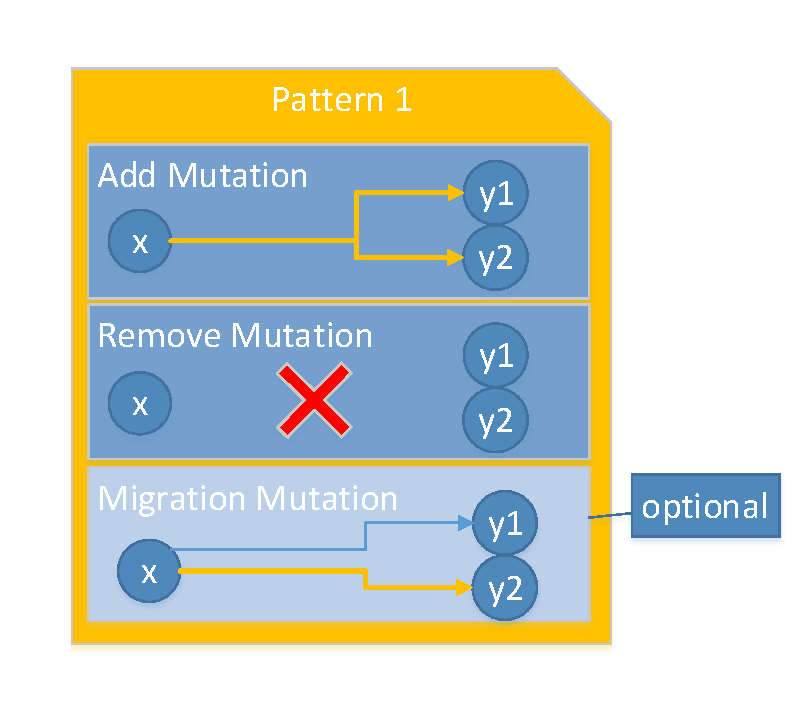
\includegraphics[scale=0.5, trim=0cm 1cm 0cm 1cm, clip=true]{Images/MutationAndFitnessFunctionDesignProcess-Step5.pdf} 
	\caption{\Gls{Mutation} and \gls{FitnessFunction} design and development process - Step 5: Define or extend \glspl{Mutation}}
	\label{figMutationAndFitnessFunctionDesignProcess-Step5}
\end{figure}

\textbf{5) Define or extend \glspl{Mutation}}: Using the pattern, the next step is to derive the actual \glspl{Mutation} (see figure \ref{figMutationAndFitnessFunctionDesignProcess-Step5}). Those are the tools of the algorithm to move through the \gls{SearchSpace}. In order to provide the algorithm the minimal ability to move back and forth, at least an add- and remove-\gls{Mutation} are required. Beyond this also more fine-grained \glspl{Mutation} are possible that enable the algorithm to make more precise moves. A \gls{Mutation} can also be associated to multiple patterns, especially remove-\glspl{Mutation}. The approach contains only a single one to remove a whole transformation rule. Since all everything else is contained in rules, this is sufficient.

Based on the example the add-\gls{Mutation} creates a transformation rule with the loop that iterates over an enumerable \gls{Property}. The remove-\gls{Mutation} is realized through the transformation rule removal \gls{Mutation}.

\begin{figure}[!ht]
	\centering
	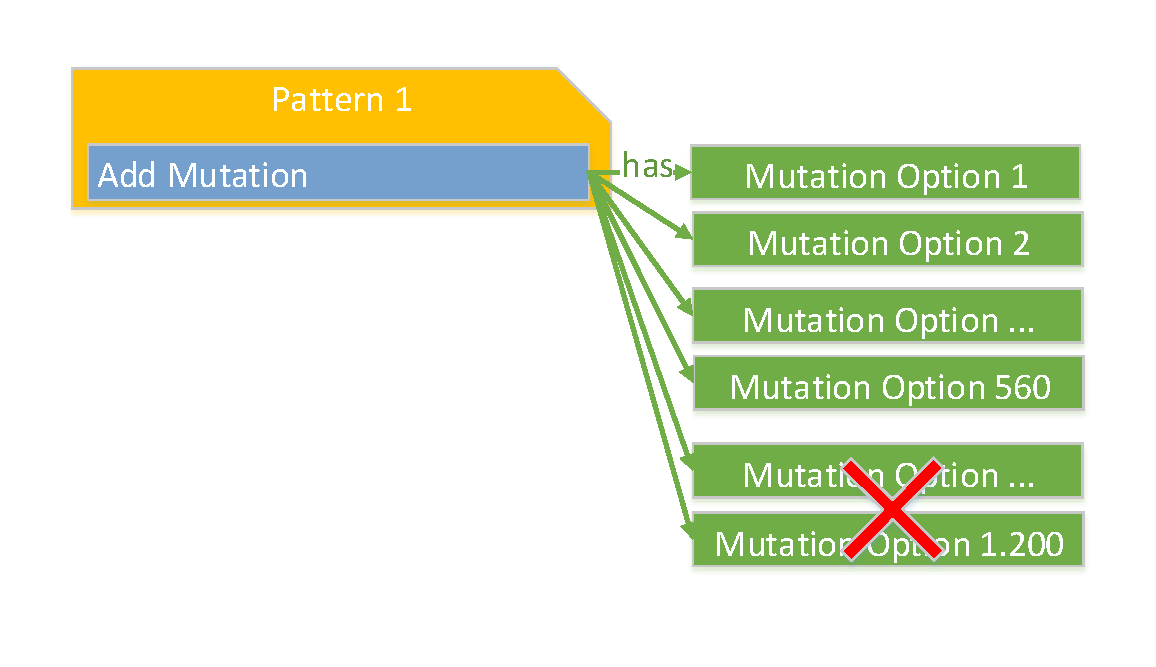
\includegraphics[scale=0.5, trim=0cm 1cm 0cm 1cm, clip=true]{Images/MutationAndFitnessFunctionDesignProcess-Step6.pdf} 
	\caption{\Gls{Mutation} and \gls{FitnessFunction} design and development process - step 6: Refine mutations}
	\label{figMutationAndFitnessFunctionDesignProcess-Step6}
\end{figure}

\textbf{6) Refine \glspl{Mutation}}: Applying the created \glspl{Mutation} in a specific context usually creates too many possible options (see figure \ref{figMutationAndFitnessFunctionDesignProcess-Step6}). The task in this step is to identify and remove options that either result in erroneous \glspl{ModelToModelTransformation} or are difficult to handle in the \gls{FitnessFunction}. Thereby, the \gls{EvolutionaryAlgorithm} less likely ends up in an unguided trial-and-error situation.

Applying the ``One-to-Many" pattern of the running example to a \gls{ModelToModelTransformation}, results in a large number of options because of the following two parameters explained. First, depending on the \glspl{MetaModel} MM$_a$ and MM$_b$, there are several possible relations of MM$_a$-MM$_b$ \glspl{Class}. Second, the possibilities for the ``Many" source are gathered by analyzing the \glspl{Property} and sub-\glspl{Property} of the MM$_a$-\gls{Class}. With this information the analysis for possible restrictions starts. The first part covering the relations of MM$_a$-MM$_b$ \glspl{Class} cannot be further reduced, but the second one can be.

Since there are several issues, only three are explained. The analysis of \glspl{Property} and sub-\glspl{Property} causes a lot of options depending on the \gls{MetaModel}. Assuming that a \gls{Property} chain like ``a.b.c.d.e" and ``a.b.c.d.f" exist. Both are enumerable \glspl{Property}, but none of them is the one which is required to create the required \glspl{Object}. Thus, the \gls{FitnessFunction} cannot distinguish between them. This is the first issue. A lot of those kind of chains are likely to exists, since in the complex scenario only one results in a valid solution. In order to avoid such a random search, an assumption about the maximum depth of the chain is added to refine the ``One-to-Many" pattern. In this context the analyzed \gls{Property} chains are of depth two, which is the minimum required to solve the given scenario.

The second issue is the possibility for self-references in the transformation rule through the enumerated \gls{Property}, which renders the whole \gls{ModelToModelTransformation} defective, since the execution cannot stop. Those options are also removed to avoid this situation.

Finally, the third issue is the one of contradictory transformations. In a situation where A is transformed into B, but at the same time A should be equivalent to C, the output is a corrupted \gls{Model} M$_b^*$. Furthermore, the manual analysis of the resulting transformation becomes difficult, hence this has to be avoided, too.

\textbf{7) Extend \glspl{FitnessFunction}}: While the \glspl{Mutation} enable the algorithm to move through the \gls{SearchSpace}, the \gls{FitnessFunction} is responsible for the guidance by rating each move. Therefore, each change of a \gls{Mutation} should be measurable by the \gls{FitnessFunction}. Ideally, a small change of a \gls{Mutation} should also cause only a small change in the result of the \gls{FitnessFunction} (see sub-section \ref{secEvolutionaryAlgorithms}). Since creating any change in the output is already difficult within the large \gls{SearchSpace} created by the \gls{TransformationLanguage}, this requirement is not applied.

%The \gls{FitnessFunction} execution has two phases. At first the comparison of the \glspl{Model} M$_b$ and M$_b^*$ results in a list of differences. Thereafter the rating of those result in a fitness value between 0 and 100 (see section \ref{secAlgorithmOverview}). Since there are several options for both, multiple \glspl{FitnessFunction} have been designed (see section \ref{secFitnessFunctions}) and evaluated (see chapter \ref{chapEvaluation}) in order to identify the differences. Adding a measurement for a \gls{Mutation} therefore requires an update of all of them.

As mentioned in step 6, the main issue dealt with in this step, is that a large fraction of the options of a \gls{Mutation} often leads to no difference in the fitness. Since the scope of the \gls{FitnessFunction} is limited to the output, there is often no possibility to change the function. If this is the case, the development needs to start over at step 4 and consider a different pattern structure, different \glspl{Mutation} or additional refinements of the \glspl{Mutation}.

\textbf{8) Implement \glspl{Mutation}}: The realization of the \glspl{Mutation} is explained in sub-section \ref{secRealizationOfMutations}.

\textbf{9) Test \glspl{Mutation} based on scenario}: Testing \glspl{Mutation} individually is important because the more are involved, the more difficult is the analysis of issues. The test of a \gls{Mutation} is based on parts of the scenarios. Thus, for each \gls{Mutation} a small test case with a \glspl{ModelToModelTransformation} as an input and output has to be created.

\begin{figure}[!ht]
	\centering
	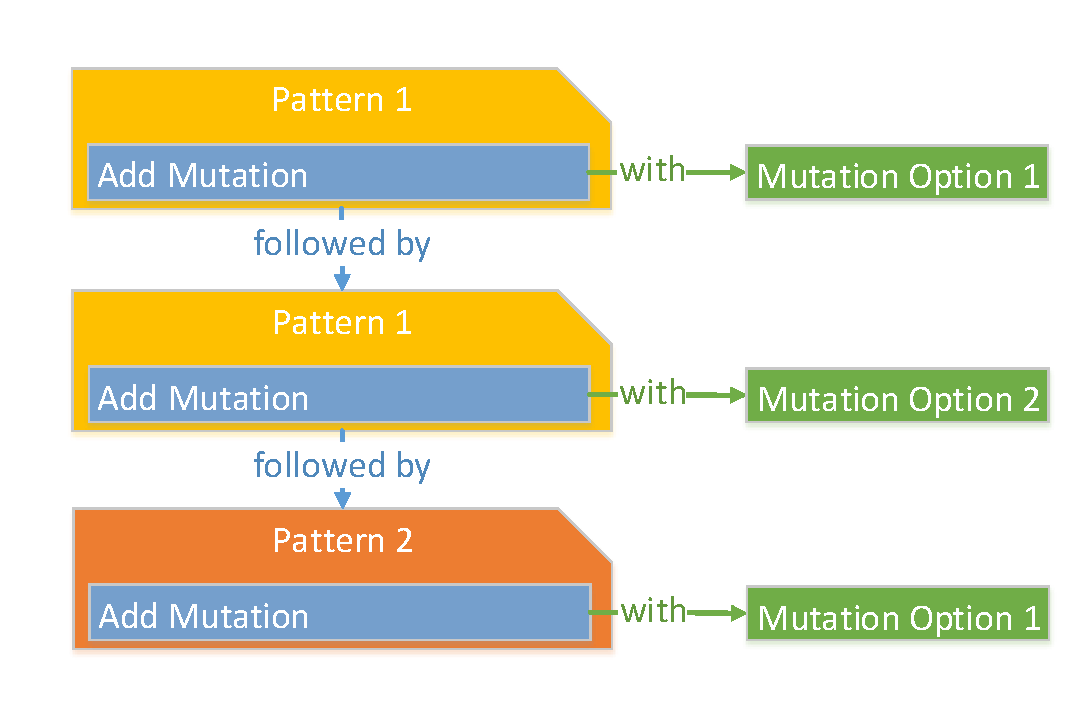
\includegraphics[scale=0.5, trim=0cm 1cm 0cm 1cm, clip=true]{Images/MutationAndFitnessFunctionDesignProcess-Step10.pdf} 
	\caption{\Gls{Mutation} and \gls{FitnessFunction} design and development process - Step 10: Test scenario construction}
	\label{figMutationAndFitnessFunctionDesignProcess-Step10}
\end{figure}

\textbf{10) Test scenario construction}: In order to ensure that the \glspl{Mutation} are able to construct the whole scenario, an integration test is required. This test is using specific \gls{Mutation} options, which represent one possibility to construct the output (see figure \ref{figMutationAndFitnessFunctionDesignProcess-Step10}). Thereby, further analysis in the evaluation phase can be simplified.

\textbf{11) Implement \glspl{FitnessFunction}}: The realization of \glspl{FitnessFunction} is explained in chapter \ref{chapPrototypeDesign}.

\textbf{12) Test \glspl{FitnessFunction} based on \glspl{Mutation}}: The \glspl{FitnessFunction} need to be tested individually based on defined scenarios. Since a complete test is difficult, only corner cases are verified. During the evaluation in the next step, control samples are be collected and added as test cases.

\textbf{13) Evaluate \glspl{Mutation} and \glspl{FitnessFunction} based on scenario(s)}: In the final step, all entities are assembled in order to verify at first that the algorithm is able to find at least any solution. Afterwards, the evaluation is started to compare and analyze the entities (see chapter \ref{chapEvaluation}). This step might also identify issues which require to re-consider the design.

For example the algorithm behaves in the first generations like a brute-force algorithm, because the \glspl{FitnessFunction} requires an identical ``Name" \gls{Property} to find an \gls{Object} match. Hence, the algorithm at first has to find the right ``Name", until any further \glspl{Association} or \glspl{Property} can be analyzed, thus ending in a situation, where only a single \gls{Mutation} option can improve the fitness. To avoid this situation a heuristic \gls{Object} comparison is added (see section \ref{secFitnessFunctions}).

\section{Transformation Pattern and Mutations}
\label{secPatternAndMutations}

\begin{figure}[htb]
	\centering
	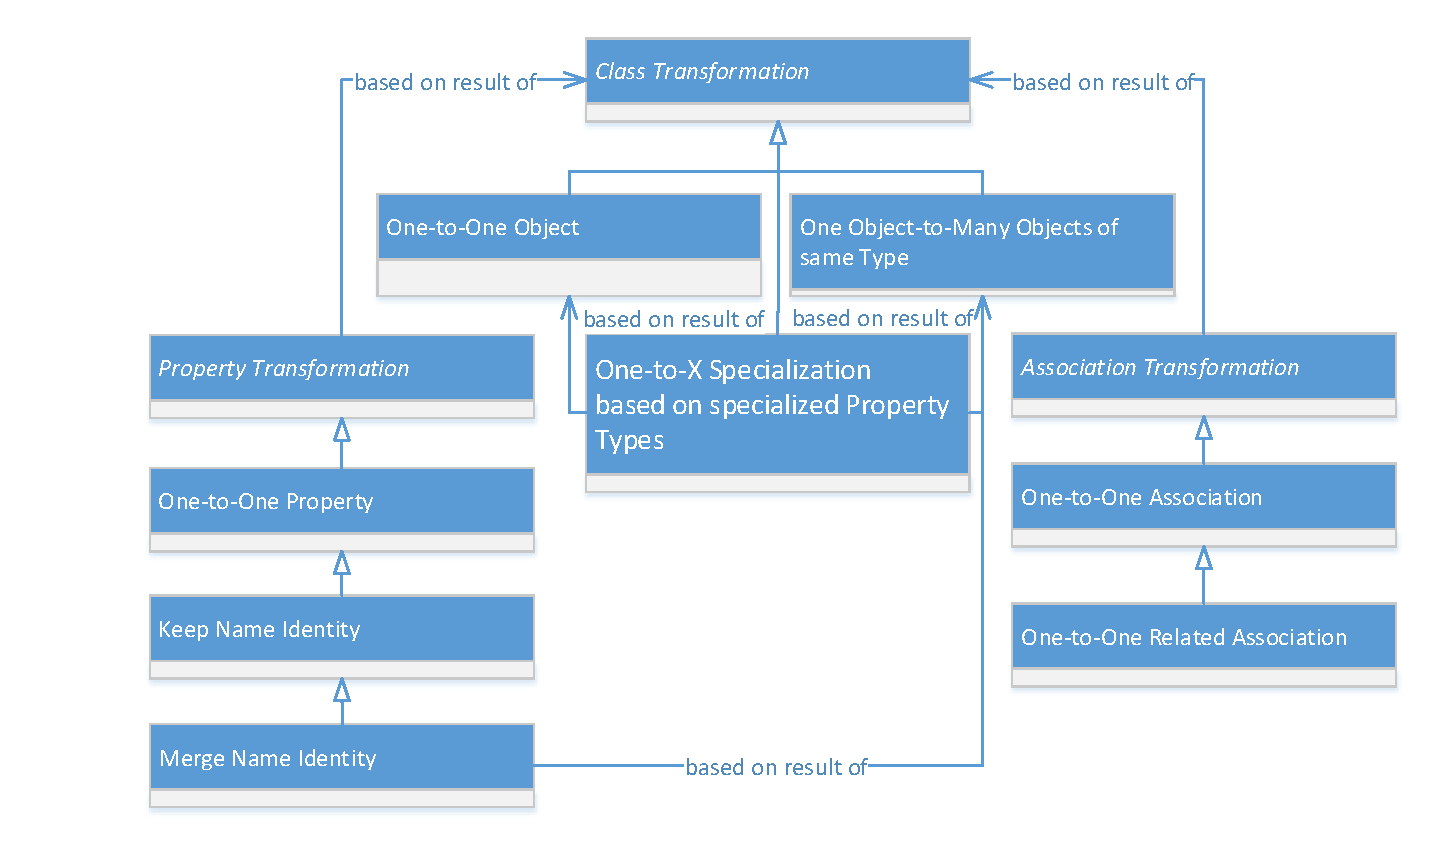
\includegraphics[scale=0.6, trim=0cm 0cm 0cm 0cm, clip=true]{Images/TransformationPattern_Overview.pdf} 
	\caption{Transformation Pattern Overview}
	\label{figTransformationPattern_Overview}
\end{figure}

In this section, the transformation pattern and the \glspl{Mutation} are presented. They are required to solve the simple and complex transformation scenario. An overview is provided in figure \ref{figTransformationPattern_Overview}. The pattern structure is derived from the conclusions of sub-section \ref{secTransformationComplexity} and the construction of the scenarios in chapter \ref{chapM2MScenarios}. The general pattern categories are \Gls{Class} Transformation, \Gls{Property} Transformation and \Gls{Association} Transformation according to the identified connect-able \glspl{Class} in the simplified \gls{MetaObjectFacility}. The pattern in these categories are described in the following subsections and have been developed according to the process described in the previous section.

As explained in the previous section, for each pattern at least an add- and one remove-\gls{Mutation} is required. The transformation pattern represents also the add-\gls{Mutation} unless otherwise stated. Since the remove-\gls{Mutation} can be coarse grained, only a single one exists which removes a whole transformation rule with all contained transformations.

\subsection{Class Transformation}
\label{secClassTransformation}

\begin{figure}[!ht]
	\centering
	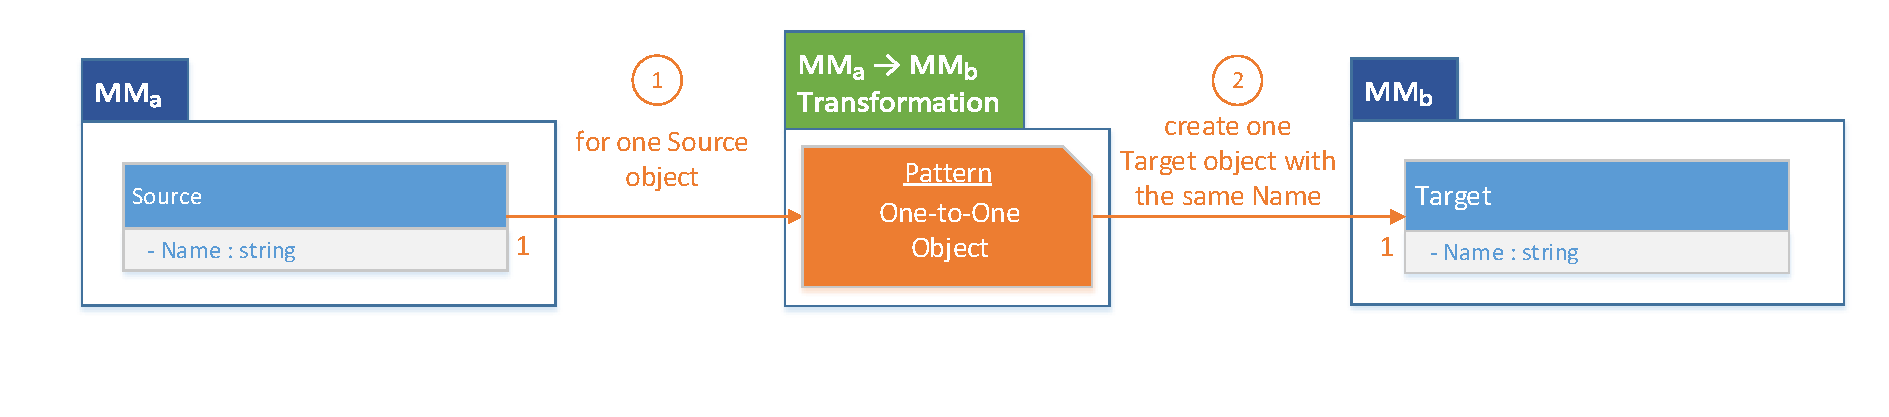
\includegraphics[scale=0.48, trim=0cm 1cm 0cm 0cm, clip=true]{Images/TransformationPattern_OneToOneObjectOfSameType.pdf} 
	\caption{Transformation Pattern: One-to-One Object}
	\label{figTransformationPattern_OneToOneObjectOfSameType}
\end{figure}

\textbf{One-to-One Object}: This is a simple, fundamental pattern required in both scenarios, which describes the transformation of one \gls{Object} of type Source from MM$_a$ into one \gls{Object} of type Target from MM$_b$ (see figure \ref{figTransformationPattern_OneToOneObjectOfSameType}). Additionally, the ``Name" \gls{Property} value is preserved. This ensures that \glspl{FitnessFunction} relying on an identical ``Name", are able to measure a difference in the output without any further \gls{Mutation}.
% - Add + Replace?: AddRuleWithNameMapping
%- Remove: RemoveRule

\begin{figure}[!ht]
	\centering
	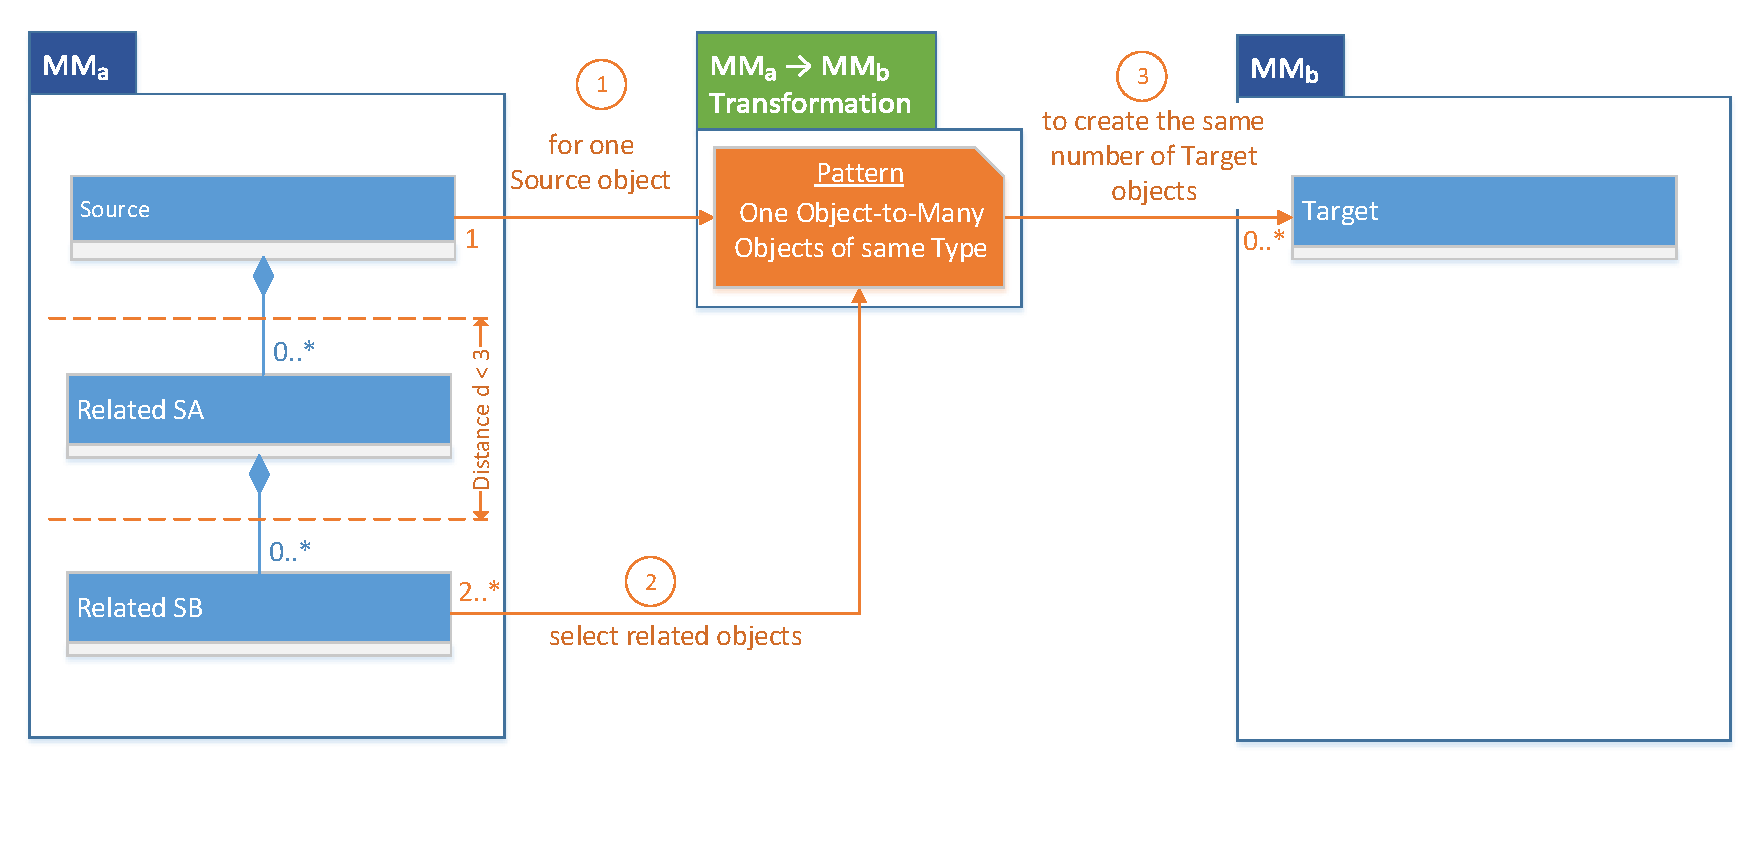
\includegraphics[scale=0.48, trim=0cm 1cm 0cm 0cm, clip=true]{Images/TransformationPattern_OneToManyObjectsOfSameType.pdf} 
	\caption{Transformation Pattern: One Object-to-Many Objects of same Type}
	\label{figTransformationPattern_OneToManyObjectsOfSameType}
\end{figure}
 
\textbf{One Object-to-Many Objects of same Type}: Transforming one \gls{Object} of type Source from MM$_a$ into several \glspl{Object} of type Target from MM$_b$ is required in the complex scenario for the outgoing transitions of a complex state which is shown in figure \ref{figTransformationPattern_OneToManyObjectsOfSameType} (see section \ref{secM2MScenarioBehavioralComplex}). In general, there are several possible sources, which define how many \glspl{Object} are created. For example, this could be defined in a \gls{Property}, calculated based on \glspl{Property}, a fixed number etc. In order to solve the complex scenario where the number of required transitions is the number of inner states, the pattern uses related \glspl{Object}. Those can be directly or indirectly related to the Source type. Since this results in a large number of options, the distance is restricted to be less than three \glspl{Association} in a row. This is the minimum number required in the complex scenario.
%  - Add: AddRuleOneToManyOfSameKind
  
\begin{figure}[!ht]
	\centering
	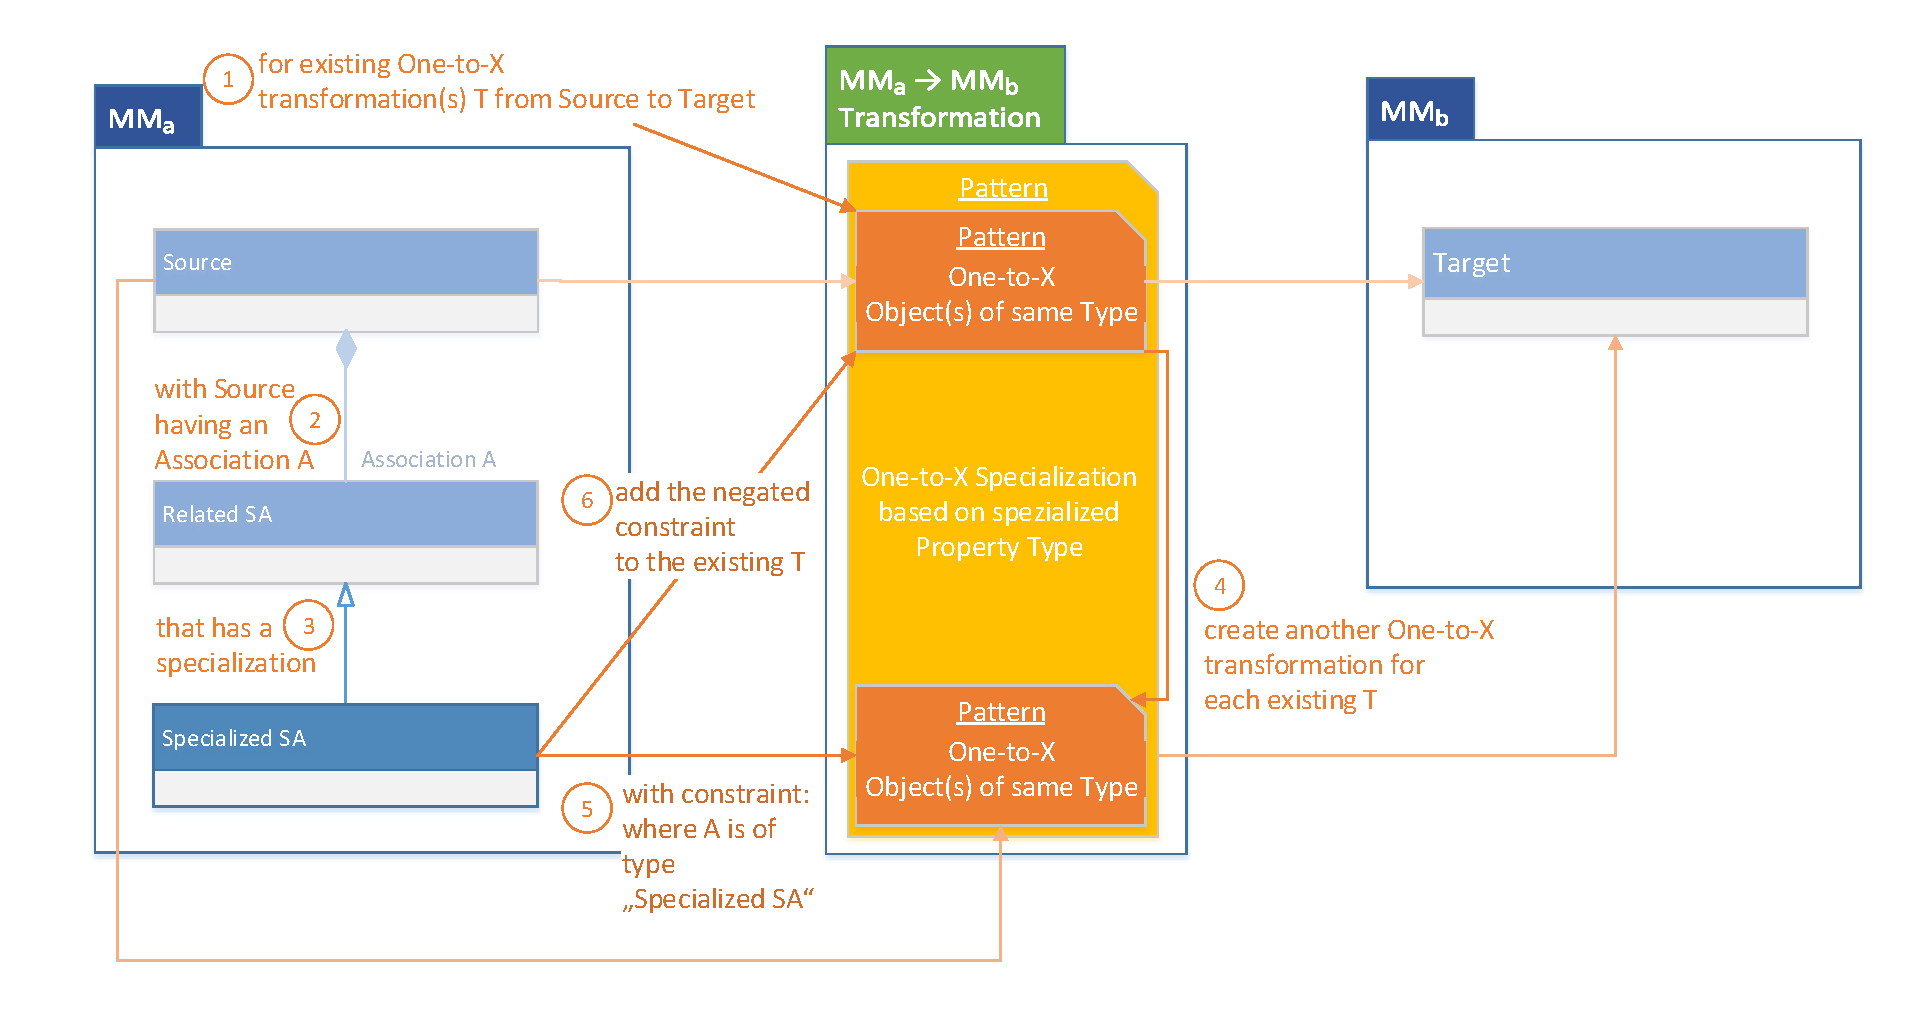
\includegraphics[scale=0.48, trim=0cm 0cm 0cm 0cm, clip=true]{Images/TransformationPattern_OneToXSpecializationBasedOnSpecializedPropertyTypes.pdf} 
	\caption{Transformation Pattern: One-to-X Specialization based on specialized Property Types}
	\label{figTransformationPattern_OneToXSpecializationBasedOnSpecializedPropertyTypes}
\end{figure} 
 
\textbf{One-to-X Specialization based on specialized Property Types}: The reference transformation for the complex scenario defines multiple Transition \glspl{TransformationRule}, depending on the context which resulted in this pattern (see section \ref{secM2MScenarioBehavioralComplex}). Using this pattern the algorithm is able to start with one of those. Afterwards, the algorithm can add the other Transition transformations step-by-step using an add-\gls{Mutation} option of this pattern. Thereby, the relevant context of a Transition is the type of the associated States. Those can be only a State or a Composite State, while the latter is a specialization of the former. For example a Transition starting at a State and ending at a Composite State has to be transformed into a Transition ending at the former Initial State of the Composite State. In the following the pattern is described in detail.

The derived concept is to take an existing \gls{TransformationRule} defined by a transformation pattern, which is cloned. Both of them are then constrained with the opposite condition. This is the foundation to achieve context specific transformations for a single type (see figure \ref{figTransformationPattern_OneToXSpecializationBasedOnSpecializedPropertyTypes}).

The pattern creates an additional transformation for the same type. Since there might be more than one context restriction, there could be also more than one existing transformation for a type. Therefore, this pattern assumes that there is a set of existing transformations which are all cloned. The second aspect is the definition of the constraint. In general, there are infinite sources for such a constraint, e.g. a \gls{Property} value or an optional \gls{Association}. In order to be able so solve the complex scenario according to the reference transformation, the derived concept is based on inheritance. Transitions in the scenario relate States, which can be Composite States since this is a sub-type. Hence, the pattern analyses the inheritance structure of the associated \glspl{Class} of type Source in MM$_a$ in a distance less than three as in the previous pattern. Whenever there is an inheritance, this is a possible constraint and thus considered as a \gls{Mutation} option.

%  - Add: SplitRuleAndAddGuardsForSuperclasses
% - Remove: RemoveRule
  
\subsection{Property Transformation} 
  
\begin{figure}[!ht]
	\centering
	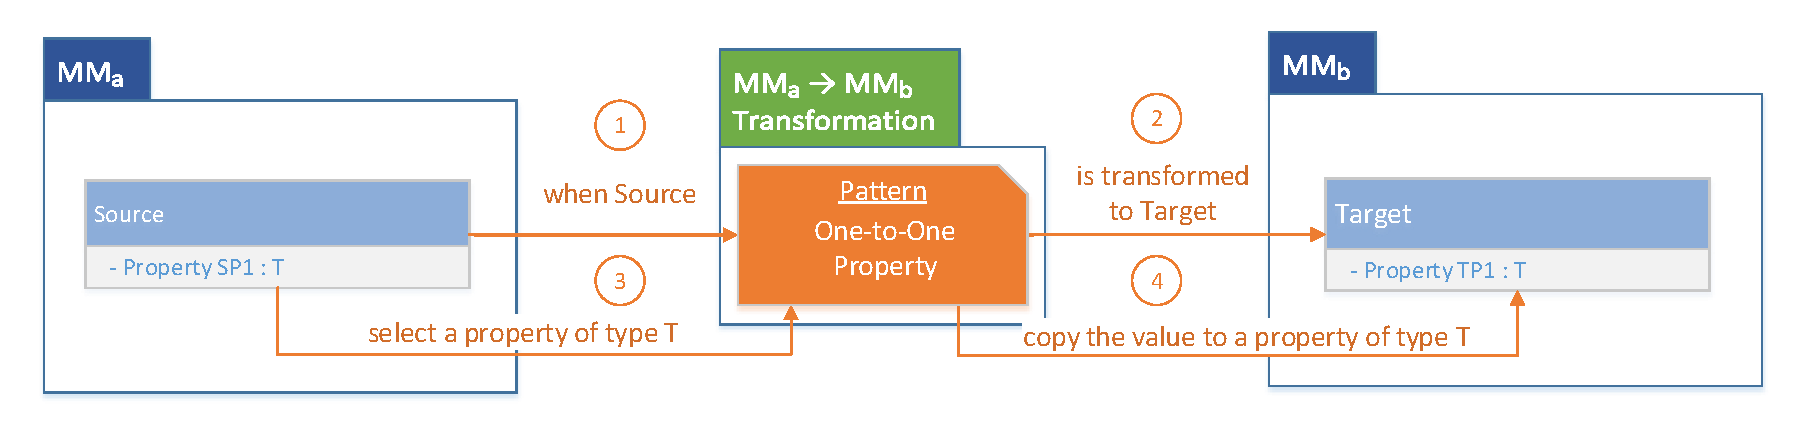
\includegraphics[scale=0.48, trim=0cm 0cm 0cm 0cm, clip=true]{Images/TransformationPattern_OneToOneProperty.pdf} 
	\caption{Transformation Pattern: One-to-One Property}
	\label{figTransformationPattern_OneToOneProperty}
\end{figure} 
 
\textbf{One-to-One Property}: Equivalent to the ``One-to-One Object" pattern on \gls{Class} level, this pattern follows the same concept on the \gls{Property} level. This pattern describes the transformation of a \gls{Property} of type Source from MM$_a$ into a \gls{Property} of the same type in Target from MM$_b$ which is required in both scenarios (see figure \ref{figTransformationPattern_OneToOneProperty}).

%  - Add + Replace:
%	- AddPropertyMapping
%	(- AddPropertyPairMapping
%	- AddRuleWithNameMapping)
%  - Remove: RemoveRule 
% => improve ``maintainability": avoid setting the same property multiple times (with different values...)
  
\begin{figure}[!ht]
	\centering
	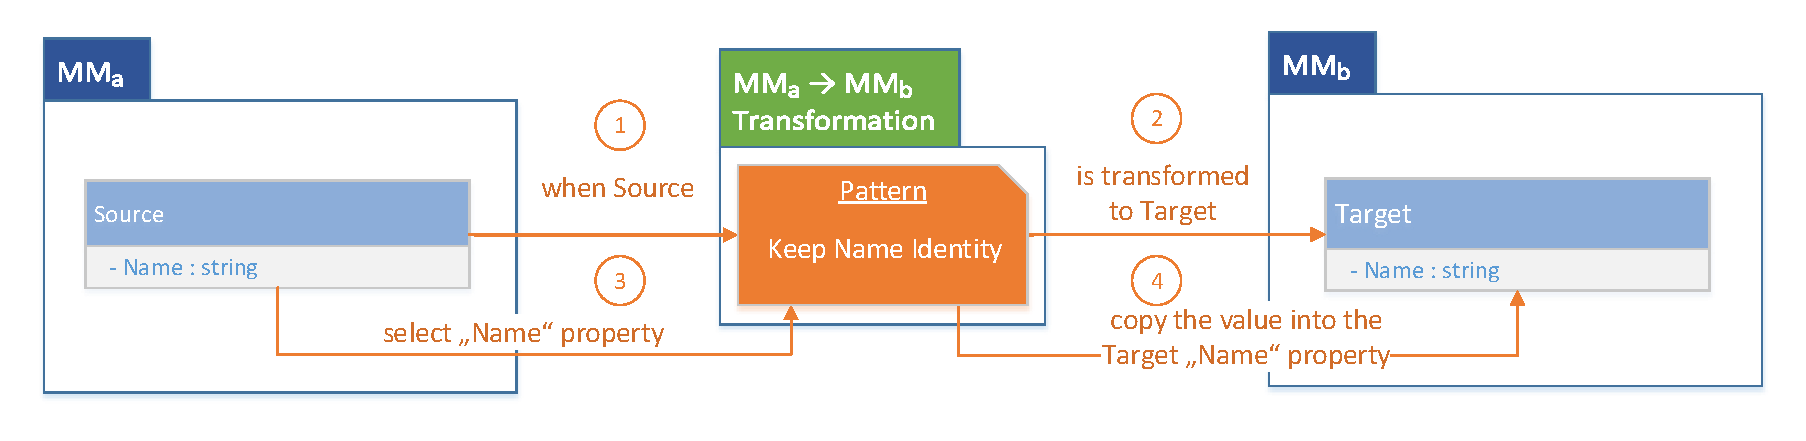
\includegraphics[scale=0.48, trim=0cm 0cm 0cm 0cm, clip=true]{Images/TransformationPattern_KeepNameIdentity.pdf} 
	\caption{Transformation Pattern: Keep Name Identity}
	\label{figTransformationPattern_KeepNameIdentity}
\end{figure} 
 
\textbf{Keep Name Identity}: Since some \glspl{FitnessFunction} require the ``Name" \gls{Property} as the identity of an \gls{Object}, this has to be kept in simple transformations. This pattern describes the conservation of the ``Name" which is required in both scenarios (see figure \ref{figTransformationPattern_KeepNameIdentity}). However, this pattern has no individual add-\gls{Mutation}, because there are two other pattern which contain this one. First, ``One-to-One Object" pattern ensures that the ``Name" is kept. Second, the ``One-to-One Property" pattern is a super set of this pattern.

%  - Add + Replace:
%	- AddRuleWithNameMapping
%	- AddPropertyMapping
%  - Remove:
%	- RemoveRule
	
\begin{figure}[!ht]
	\centering
	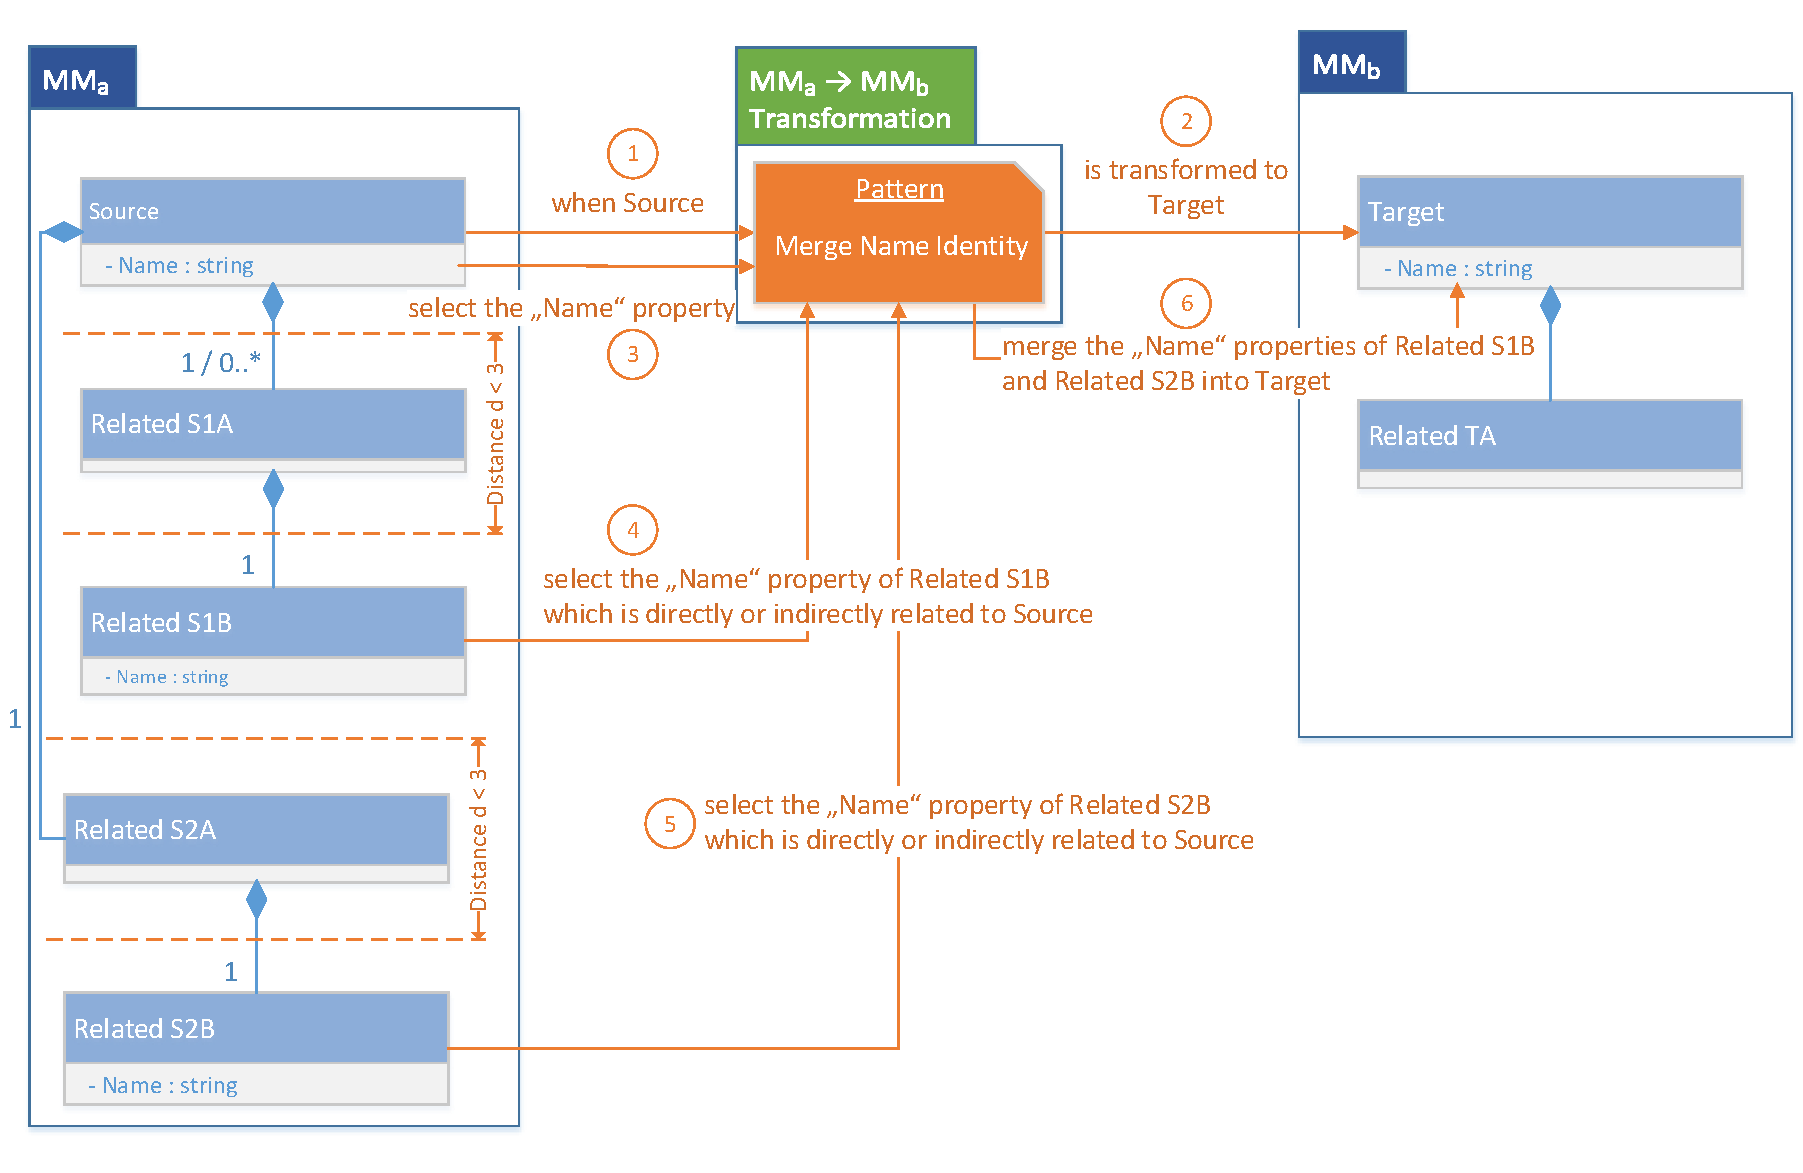
\includegraphics[scale=0.48, trim=0cm 0cm 0cm 0cm, clip=true]{Images/TransformationPattern_MergeNameIdentity.pdf} 
	\caption{Transformation Pattern: Merge Name Identity}
	\label{figTransformationPattern_MergeNameIdentity}
\end{figure} 
 
\textbf{Merge Name Identity}: Besides having to keep the ``Name" \gls{Property}, there are situations in the complex scenario where it is not that simple. Transitions describe the connection of two States and hence their ``Name" is based on this relationship like ``State1 $\rightarrow$ State2". In the case this relationship changes, the name has to be changed, too. The more general concept is to define the ``Name" based on associated \glspl{Object} which results into this pattern (see figure \ref{figTransformationPattern_MergeNameIdentity}). Similar to the ``One Object-to-Many Objects of same Type" pattern, the context is analyzed in a distance less than three and pairs of \glspl{Object} are created as \gls{Mutation} options. The ``Name" of each pair is used to assemble a new ``Name" in the form ``Name1 $\rightarrow$ Name2". Referring to section \ref{secTransformationComplexity}, this is a calculated \gls{Property}.

%  - Add + Replace:
%	- AddPropertyPairMapping
%  - Remove:
%	- RemoveRule

\subsection{Association Transformation} 	
  
\begin{figure}[!ht]
	\centering
	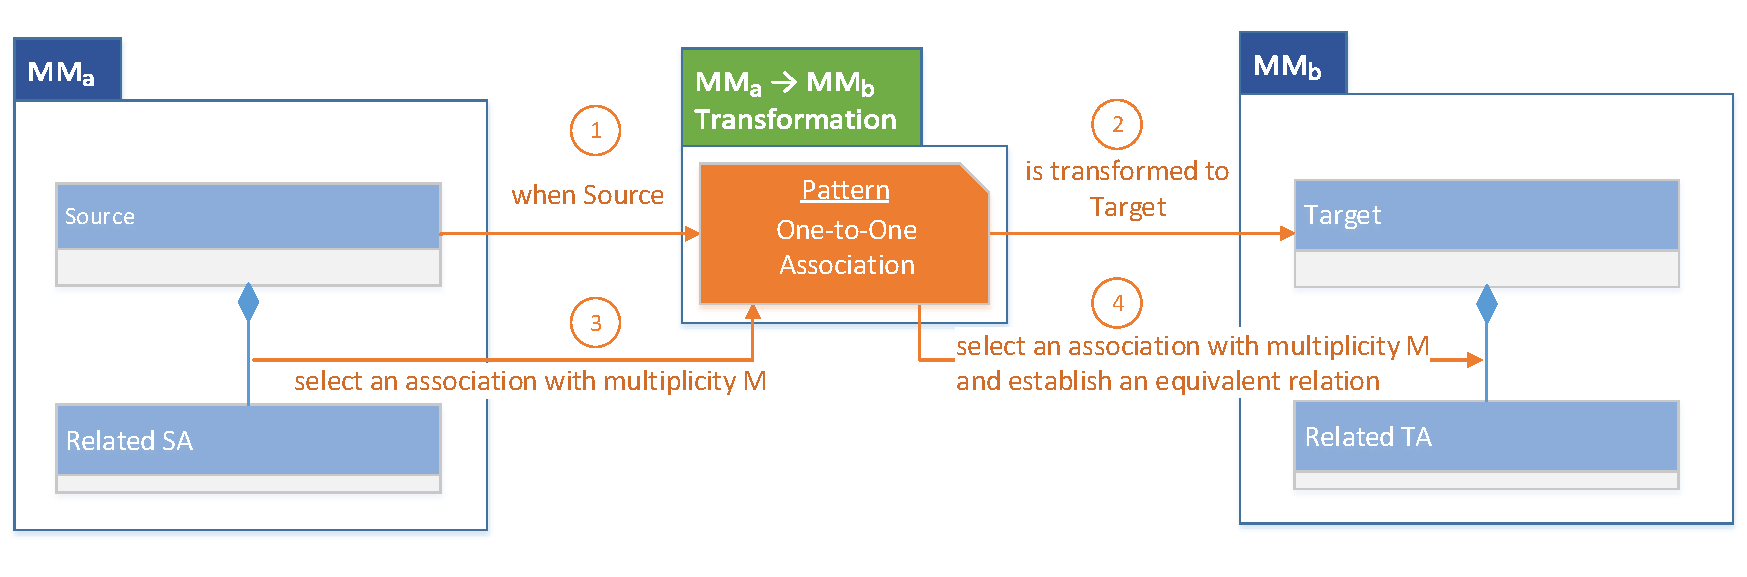
\includegraphics[scale=0.48, trim=0cm 0cm 0cm 0cm, clip=true]{Images/TransformationPattern_OneToOneAssociation.pdf} 
	\caption{Transformation Pattern: One-to-One Association}
	\label{figTransformationPattern_OneToOneAssociation}
\end{figure}

\textbf{One-to-One Association}: As already observed on the \gls{Class} and \gls{Property} level, the first pattern is the transformation of a single \gls{Association} of the Source type from MM$_a$. It is transformed into a single \gls{Association} with the same multiplicity of the Target type from MM$_b$ (see figure \ref{figTransformationPattern_OneToOneAssociation}). Both scenarios require this pattern, but it does not have an individual add-\gls{Mutation} since \glspl{Association} relate \glspl{Property} according to the simplified \gls{MetaObjectFacility} (see sub-section \ref{secModelLanguage}). Hence, the add-\gls{Mutation} of the ``One-to-One Property" pattern is used.

%  - Add + Replace:
%	- AddPropertyMapping
%  - Remove: RemoveRule
  
\begin{figure}[!ht]
	\centering
	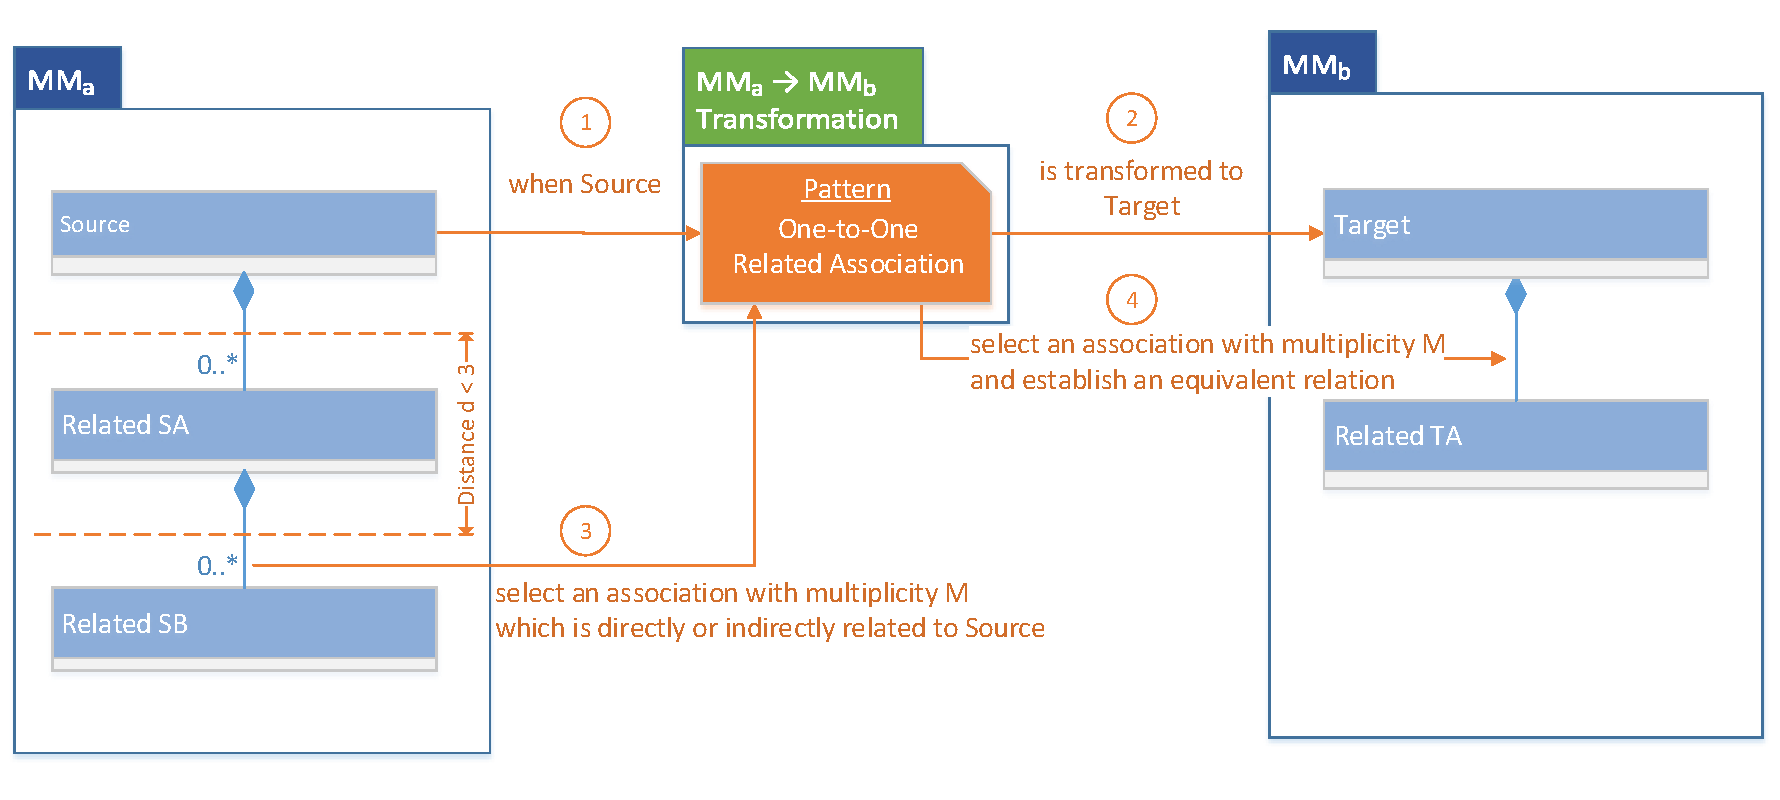
\includegraphics[scale=0.48, trim=0cm 0cm 0cm 0cm, clip=true]{Images/TransformationPattern_OneToOneRelatedAssociation.pdf} 
	\caption{Transformation Pattern: One-to-One Related Association}
	\label{figTransformationPattern_OneToOneRelatedAssociation}
\end{figure}

\textbf{One-to-One Related Association}: In the complex scenario the Transitions pointing to a complex state have to be replaced by Transitions pointing to the Initial State of the Complex State (see section \ref{secM2MScenarioBehavioralComplex}). The derived pattern is to transform an indirectly related \gls{Association} of the Source type from MM$_a$ into a directly related \gls{Association} of the Target type from MM$_b$ (see figure \ref{figTransformationPattern_OneToOneAssociation}). The distance is limited to less than three in order to avoid the excessive creation of \gls{Mutation} options as already in similar previous pattern. 

%  - Add + Replace:
%	- AddPropertyMapping
%  - Remove: RemoveRule 
   
%  => justify requirement by referring to scenarios - matrix? meta model??

%Mutations:
%- AddPropertyMapping
%- AddPropertyPairMapping
%- AddRuleOneToManyOfSameKind
%- AddRuleWithNameMapping
%- RemoveRule
%- SplitRuleAndAddGuardsForSuperclasses

\section{Fitness Functions}
\label{secFitnessFunctions}

The \gls{FitnessFunction} execution has two phases shown in listing \ref{lstFitnessEvaluatorOverview}. At first, the comparison of the \glspl{Model} M$_b$ and M$_b^*$ using the ``Comparator" results in a list of differences. Those are aggregated within a ``Comparison" to the number of matched \glspl{Class}, \glspl{Property} and \glspl{Association}. Thereafter, the rating of those results in a fitness value between 0\% and 100\% (see section \ref{secAlgorithmOverview}). The fitness value is thereby calculated using a weighted function. Since there are several options for the ``Comparator" and the ``Weights", multiple \glspl{FitnessFunction} have been designed and evaluated (see chapter \ref{chapEvaluation}) in order to identify the differences.

\begin{lstlisting}[language=PSEUDO,caption={Overview of fitness evaluation in pseudo code},label={lstFitnessEvaluatorOverview},mathescape]
module FitnessEvaluator {
	evaluate($M_b$, $M_b^*$, Comparator comparator, Weights weights) {
	
		// Phase 1: Object graph comparison
		Comparison comparison = comparator.compare($M_b$, $M_b^*$)
		
		// Phase 2: use the defined fitness function to compute the fitness
		return fitness(weights, comparison)	
	}
}
\end{lstlisting}

In the following the used comparison methods are presented in sub-section \ref{secObjectGraphComparisonMethods}, the generic \gls{FitnessFunction} in sub-section \ref{secGenericFitnessFunction} and the used configurations in sub-section \ref{secFitnessFunctionConfigurations}.

%$$compare(m, v; M_b, M_b^*)$$

%\begin{align*}
%  \text{where}~m &= \{nameidentity,heuristic,nameidentitywithheuristicfallback\} \\
%  v &= \{{c_f},{c_e},{p_f},{a_f}\}\\
%\end{align*}


%$$fitness(M_b, M_b^*, m, c_w, c_{we}, p_w, a_w) = $$
%$$fitness(c_w,compare(m,c_f;M_b, M_b^*),compare(m,c_e;M_b, M_b^*),p_w,compare(m,p_f;M_b, M_b^*),a_w,compare(m,a_f;M_b, M_b^*))$$


\subsection{Object Graph Comparison Methods}
\label{secObjectGraphComparisonMethods}

Comparing the \gls{Object} graphs of M$_b$ and M$_b^*$ is realized in three ways. The first ``Name identity" comparison is based on the assumption that every \gls{Object} is identified by a unique ``Name" \gls{Property}. This is assumption does not hold for any scenario, but for the presented ones. The second comparison approach is based on a heuristic matching. It compares \glspl{Object} based on their \glspl{Association} and \glspl{Property} and is defined within EMF Compare (see \cite{EclipseFoundation2014b}). In the following it is referred to as ``Heuristic". Finally, the third comparison method ``Name identity with heuristic fall-back" is a combination of the two. It matches \glspl{Object} based on the ,,Name" and if there is no result, uses the heuristic as a fall-back. The heuristic is derived from \cite{EclipseFoundation2014c} and presented in the following.

The $distance(a,b)$ between two \glspl{Object} a and b is the sum of all \gls{Property} changes $c(p)$. Whereas primitive \gls{Property} changes, which are only "Name" \gls{Property} changes in both scenarios, have a higher weight $w(p)$ than \gls{Association} changes. These values have been determined empirically by \cite{EclipseFoundation2014c}. Changes of string \glspl{Property} are measured by the Dice Coefficient \cite{Jaccard1912} similarity function. It results in more granular increments for those. In both scenarios this is applied to the "Name" \gls{Property}. Whereas only in the complex scenario is an increment when creating the new Transitions with the "Merge Name Identity" pattern. The comparison of associated \glspl{Object} is performed by the $simplematch(a,b)$ function, which compares the type and the index. The latter is a heuristic based on the assumption that the order of the \glspl{Object} in M$_b$ and M$_b^*$ are identical.

% recursion, top down / level by level anaylsis...

$$distance(a,b) = \sum_{p \in P_{a,b}} w(p) c(p,a,b) $$

\begin{align*}
  \text{where}~
	w(p) &= \left\{
				\begin{array}{l l}
					5 & \quad \text{if $p$ is primitive}\\
					2 & \quad \text{if $p$ is member of an association}
				\end{array}\right.\\		   
	c(p) &= \left\{
				\begin{array}{l l}	
					1 - dice(a(p),b(p)) & \quad \text{if $p$ is string}\\				
					1 & \quad \text{if p is primitive and $a(p) \neq b(p)$}\\
					1 & \quad \text{if not $simplematch(a(p),b(p))$ }\\			
					0 & \quad \text{else}
				\end{array}\right.\\
	simplematch(a,b) &= (typeof(a) = typeof(b)) \land (indexof(a) = indexof(b))
\end{align*}

In order to determine, if two \glspl{Object} are equal at all, the maximum distance function $maxdistance(a,b)$ is used to filter out pairs with too many differences. The maximum is computed as the sum of all weighted \glspl{Property}, which is the largest distance. This is reduced by an empirically determined factor (see \cite{EclipseFoundation2014c}) depending on the number of \glspl{Property} $i$ in $threshold(i)$:

$$maxdistance(a,b) = threshold(|\{p \in P_{a,b}\}|) \sum_{p \in P_{a,b}} w(p)$$

\begin{align*}
  \text{where}~
	threshold(i) &= \left\{
				\begin{array}{l l}
					0 & \quad \text{if $i < 1$}\\
					0.6 & \quad \text{if $i < 3$}\\
					0.55 & \quad \text{if $i < 4$}\\
					0.465 & \quad \text{else}
				\end{array}\right.
\end{align*}

The equivalent \gls{Object} b for a given \gls{Object} a is one of the \glspl{Object} with the minimum distance. A distance is infinite in the case it is larger than the maximum distance:

$$match(a, {b_1,..,b_n}) = \min_{b \in {b_1,..,b_n}} matchdistance(a,b) $$

\begin{align*}
  \text{where}~
	matchdistance(a,b) &= \left\{
				\begin{array}{l l}
					distance(a,b) & \quad \text{if $distance(a,b) <$ } \\ 
					& \quad \text{$maxdistance(a,b)$}\\
					infinite & \quad \text{else}
				\end{array}\right.
\end{align*}


%- attrribute only "Name"
%- references equivalent by order in output
%- root must have the correct name and contain the rest.. (EMF)

%weight per change:
%	referenceChange = 2
%	attributeChange = 5
%	* 1 / "name" = 4 / "id" = 4 / reference = 2
%
%	if move: * orderChange = 1
%	if change of string -> string: * 1 - dice coefficient
%	
%	====
%	
%	if already changed --> 1 (!!))
	
	
%distance = sum all weights

%maxDistance = sum of weights of attributes with values * 0.465d

%if < maxDistance => identical

%Therefore the EMF Compare Edition Distance Function 


%EmfCompare
%\cite{EclipseFoundation2014b}
%\cite{Toulme2006}

%ProximityEObjectMatcher

%EditionDistance - ReflectiveWeightProvider (assoc diff larger distance than props), DefaultDiffEngine

%--> the distance between them computed using the number of changes required to change a to b.

%- eContainingFeature different?
%	- must not be greater than the max distance (max Distance (empirical): based on number of features, with some empirically gathered weights)
%	-> then detailed measurement:
%		- order of features is measured
%		- equality of strings measured with dice coefficient of two string's bigrams
%		- creates longest common susequence of matching props, assoc
%		- "id" and "name" have a bigger effect than other properties


\subsection{Generic Fitness Function}
\label{secGenericFitnessFunction}

The differences between M$_b$ and M$_b^*$ determined by the methods described in the previous sub-section are the foundation for the actual \gls{FitnessFunction}. This sub-section presents a generic function with several weights rendering it configurable. Those are explained in the following sub-section \ref{secFitnessFunctionConfigurations}.

According to the simplified \gls{MetaObjectFacility} (see sub-section \ref{secModelLanguage}), the instantiated \gls{MetaObjectFacility} \glspl{Class} of M$_b$ and M$_b^*$ are \glspl{Class}, \glspl{Property} and \glspl{Association}. Hence, those define the structure of the fitness function, which compares the matched elements with the expected ones in those categories. As explained, weights must be defined for each of the three \gls{MetaObjectFacility} \glspl{Class}:

$$fitness(c_w,c_f,c_e,p_w,p_f,a_w,a_f) = \frac{c_w c_f - c_{we} c_e + p_w p_f + a_w a_f}{c_w + p_w + a_w}$$

\begin{align*}
  \text{where}~c_w &= \text{weight of ``\gls{Class} fitness"}, \\
  c_f &= \frac{c_{matched}}{c_{expected}}\% = \text{``\gls{Class} fitness"},\\
  c_{we} &= \text{weight of ``\gls{Class} error"}, \\
  c_e &= \frac{c_{unexpected}}{c_{created}}\% = \text{``\gls{Class} error"}, \\  
  p_w &= \text{weight of ``Primitive \gls{Property} fitness"}, \\
  p_f &= \frac{p_{matched}}{p_{expected}}\% = \text{``Primitive \gls{Property} fitness"},\\ 
  a_w &= \text{weight of ``\gls{Association} \gls{Property} fitness"}, \\
  a_f &= \frac{a_{matched}}{a_{expected}}\% = \text{``\gls{Association} \gls{Property} fitness"},\\
%  a_{we} &= \text{weight of ``\gls{Association} error"}, \\
%  a_e &= \frac{a_{unexpected}}{a_{created}}\% = \text{``\gls{Association} error"},\\
  \text{with}~& c_w \geq c_{we} %\land a_w \geq a_{we}
\end{align*}

Since \gls{Class} instances - \glspl{Object} - are not limited by the \gls{MetaModel}, there can be unexpected ones in M$_b^*$ which cannot be matched in M$_b$. Without any penalty in the function, the algorithm identifies \glspl{ModelToModelTransformation} as solution that create every combination of e.g. Transitions. Thus, those falsely transformed \glspl{Object} reduce the fitness in order to create a penalty and guide the algorithm in the desired way. \Glspl{Association} with an unlimited multiplicity cause such an issue, but since they are only measured through the \glspl{Property}, this error is not included in the function. %as well as \glspl{Association} with an unlimited multiplicity => associations are not evaluated in detail, just "is the property correct"

% - penalty for wrong rules and property mappings (or added constructs that cause no fitness change !?)

\subsection{Fitness Function Configurations}
\label{secFitnessFunctionConfigurations}

The previous subsections defined the comparison methods and the generic fitness function. In this section the used configurations are presented. Those are defined based on the pseudo code of the fitness evaluation shown in listing \ref{lstFitnessEvaluator}, which is an extension of listing \ref{lstFitnessEvaluatorOverview}. On the one hand, the ``Comparator" has the three realizations ``NameIdentity", ``Heuristic" and ``NameIdentityWithHeuristicFallback" (see subsection \ref{secObjectGraphComparisonMethods}). On the other hand, the ``fitness" function requires also the ``Weights" defined in subsection \ref{secGenericFitnessFunction}.

%structure Comparison {
%	attribute $c_{matched}$
%	attribute $c_{expected}$
%	attribute $c_{unexpected}$
%	attribute $c_{created}$
%	attribute $p_{matched}$
%	attribute $p_{expected}$
%	attribute $a_{matched}$
%	attribute $a_{expected}$	
%}
\begin{lstlisting}[language=PSEUDO,caption={Fitness evaluation in pseudo code},label={lstFitnessEvaluator},mathescape]
interface Comparator {
	compare($M_b$, $M_b^*$) returns Comparison;
}

module NameIdentity realizes Comparator {
	... // identifies equal objects based on their name
}

module Heuristic realizes Comparator {
	... // identifies equal objects based on the defined heuristic
}

module NameIdentityWithHeuristicFallback realizes Comparator {
	... // identifies equal objects based on their name.
		  // if their is no match, it uses the defined heuristic
}

structure Weights {
	attribute $c_w$
	attribute $c_{we}$
	attribute $p_w$
	attribute $a_w$
}

module FitnessEvaluator {
	evaluate($M_b$, $M_b^*$, Comparator comparator, Weights weights) {
	
		// Phase 1: Object graph comparison
		Comparison comparison = comparator.compare($M_b$, $M_b^*$)
		
		// Phase 2: use the defined fitness function to compute the fitness
		return fitness(weights, comparison)	
	}
}
\end{lstlisting}

The following \gls{FitnessFunction} configurations are defined based on the comparison methods and function weights. Since there are infinite weights assignable, it is not possible to create all configurations. Hence, a few are selected in this sub-section and evaluated in chapter \ref{chapEvaluation}.

%BalancedFitnessFunction
\textbf{Class focused using Name}: A correct \gls{Class} transformation is a prerequisite for the analysis of further transformations. This is especially crucial, when using the ``Name identity" comparison method. This configuration focuses the algorithm on the identification of \gls{Class} at first. It is expected that having a correct \gls{Class} transformation at first is useful, since any change of such a transformation has an impact on the contained \glspl{Property} and related \glspl{Association}. Thus, changing an existing \gls{Class} transformation reverts all related changes as well.

$$evaluate(M_b, M_b^*, Comparator, Weights)$$
\begin{align*}
  \text{where}~Comparator &= \text{NameIdentity}, \\
  Weights.c_w &= \text{2}, \\
  Weights.c_{we} &= \text{1}, \\
  Weights.p_w &= \text{1}, \\
  Weights.a_w &= \text{1} \\
\end{align*}

%StructureFocusedFitnessFunction
\textbf{More class focused using Name}: In order to evaluate the relevance of assigning \glspl{Class} more weight, this configuration increases the difference compared to the first one.

$$evaluate(M_b, M_b^*, Comparator, Weights)$$
\begin{align*}
  \text{where}~Comparator &= \text{NameIdentity}, \\
  Weights.c_w &= \text{10}, \\
  Weights.c_{we} &= \text{1}, \\
  Weights.p_w &= \text{1}, \\
  Weights.a_w &= \text{1} \\
\end{align*}

%BalancedFitnessFunctionBasedOnlyOnStructure
\textbf{Class focused using heuristic}: Evaluating the difference between the ,,Heuristic" comparison method and the two others requires this configuration.

$$evaluate(M_b, M_b^*, Comparator, Weights)$$
\begin{align*}
  \text{where}~Comparator &= \text{Heuristic}, \\
  Weights.c_w &= \text{2}, \\
  Weights.c_{we} &= \text{1}, \\
  Weights.p_w &= \text{1}, \\
  Weights.a_w &= \text{1} \\
\end{align*}

%BalancedFitnessFunctionBasedOnStructureAsFallback
\textbf{Class focused using Name and heuristic fall-back}: Evaluating the difference between the ,,Name identity with heuristic fall-back" comparison method and the two others requires this configuration.

$$evaluate(M_b, M_b^*, Comparator, Weights)$$
\begin{align*}
  \text{where}~Comparator &= \text{NameIdentityWithHeuristicFallback}, \\
  Weights.c_w &= \text{2}, \\
  Weights.c_{we} &= \text{1}, \\
  Weights.p_w &= \text{1}, \\
  Weights.a_w &= \text{1} \\
\end{align*}

%BalancedFitnessFunctionBasedOnStructureAsFallbackAndImportantAssociations
\textbf{Class and association focused using name and heuristic fall-back}: Since the heuristic utilized the \glspl{Association} in order to transform \glspl{Class}, this configuration increases the weight for those, too.

$$evaluate(M_b, M_b^*, Comparator, Weights)$$
\begin{align*}
  \text{where}~Comparator &= \text{NameIdentityWithHeuristicFallback}, \\
  Weights.c_w &= \text{2}, \\
  Weights.c_{we} &= \text{1}, \\
  Weights.p_w &= \text{1}, \\
  Weights.a_w &= \text{2} \\
\end{align*}

%PropertyFocusedFitnessFunctionBasedOnStructureAsFallback
\textbf{Property focused using Name and heuristic fall-back}: In order to provide a counter-example for the \gls{Class} emphasis, this configuration is defined.

$$evaluate(M_b, M_b^*, Comparator, Weights)$$
\begin{align*}
  \text{where}~Comparator &= \text{NameIdentityWithHeuristicFallback}, \\
  Weights.c_w &= \text{1}, \\
  Weights.c_{we} &= \text{1}, \\
  Weights.p_w &= \text{3}, \\
  Weights.a_w &= \text{3} \\
\end{align*}

%- BalancedFitnessFunction
%		double mofClassFitness = (maximumFitness / numberOfMofClassInstancesInManuallyCreatedModel) * (numberOfMofClassInstancesInManuallyCreatedModel - numberOfnotMappedMofClassInstances);
%		double mofClassError = numberOfMofClassInstancesInOutputModelOfIndividual > 0 ? (numberOfunexpectedMappedMofClassInstances / numberOfMofClassInstancesInOutputModelOfIndividual) * maximumFitness : 0;
%		double mofPropertyFitness = (maximumFitness / numberOfMofPropertiesInManuallyCreatedModel) * (numberOfMofPropertiesInManuallyCreatedModel - (numberOfNotMappedMofPropertiesInNotMappedClasses + numberOfnotMappedMofPropertiesInMappedMofClassesWithAssociations));
%
%		double fitness = (mofClassFitness * 2 - mofClassError + mofPropertyFitness) / 3.;
%		return fitness < 0. ? 0. : fitness;
%
%- BalancedFitnessFunctionBasedOnlyOnStructure
%- BalancedFitnessFunctionBasedOnStructureAsFallback
%
%- BalancedFitnessFunctionBasedOnStructureAsFallbackAndImportantAssociations
%		double mofClassFitness = (maximumFitness / numberOfMofClassInstancesInManuallyCreatedModel) * (numberOfMofClassInstancesInManuallyCreatedModel - numberOfnotMappedMofClassInstances);
%		double mofClassError = numberOfMofClassInstancesInOutputModelOfIndividual > 0 ? (numberOfunexpectedMappedMofClassInstances / numberOfMofClassInstancesInOutputModelOfIndividual) * maximumFitness : 0;
%
%		int numberOfMofPropertiesInManuallyCreatedModelExcludingAssocations = numberOfMofPropertiesInManuallyCreatedModel - numberOfMofAssociationPropertiesInManuallyCreatedModel;
%		int numberOfNotMappedMofPropertiesInNotMappedClassesExcludingAssociations = numberOfNotMappedMofPropertiesInNotMappedClasses - numberOfNotMappedMofAssociationPropertiesInNotMappedClasses;
%		int numberOfnotMappedMofPropertiesInMappedMofClassesExcludingAssociations = numberOfnotMappedMofPropertiesInMappedMofClassesWithAssociations - numberOfnotMappedMofAssociationPropertiesInMappedMofClasses;
%		double mofPropertyFitness = (maximumFitness / numberOfMofPropertiesInManuallyCreatedModelExcludingAssocations)
%				* (numberOfMofPropertiesInManuallyCreatedModelExcludingAssocations - (numberOfNotMappedMofPropertiesInNotMappedClassesExcludingAssociations + numberOfnotMappedMofPropertiesInMappedMofClassesExcludingAssociations));
%		double mofAssociationPropertyFitness = (maximumFitness / numberOfMofAssociationPropertiesInManuallyCreatedModel)
%				* (numberOfMofAssociationPropertiesInManuallyCreatedModel - (numberOfNotMappedMofAssociationPropertiesInNotMappedClasses + numberOfnotMappedMofAssociationPropertiesInMappedMofClasses));
%
%		double fitness = (mofClassFitness * 2 - mofClassError + mofAssociationPropertyFitness * 2 + mofPropertyFitness) / 5.;
%		return fitness < 0. ? 0. : fitness;
%
%- PropertyFocusedFitnessFunctionBasedOnStructureAsFallback
%		double mofClassFitness = (maximumFitness / numberOfMofClassInstancesInManuallyCreatedModel) * (numberOfMofClassInstancesInManuallyCreatedModel - numberOfnotMappedMofClassInstances);
%		double mofClassError = numberOfMofClassInstancesInOutputModelOfIndividual > 0 ? (numberOfunexpectedMappedMofClassInstances / numberOfMofClassInstancesInOutputModelOfIndividual) * maximumFitness : 0;
%		double mofPropertyFitness = (maximumFitness / numberOfMofPropertiesInManuallyCreatedModel) * (numberOfMofPropertiesInManuallyCreatedModel - (numberOfNotMappedMofPropertiesInNotMappedClasses + numberOfnotMappedMofPropertiesInMappedMofClassesWithAssociations));
%
%		double fitness = (mofClassFitness - mofClassError + mofPropertyFitness * 3) / 4.;
%		return fitness < 0. ? 0. : fitness;
%- StructureFocusedFitnessFunction
%		double mofClassFitness = (maximumFitness / numberOfMofClassInstancesInManuallyCreatedModel) * (numberOfMofClassInstancesInManuallyCreatedModel - numberOfnotMappedMofClassInstances);
%		double mofClassError = numberOfMofClassInstancesInOutputModelOfIndividual > 0 ? (numberOfunexpectedMappedMofClassInstances / numberOfMofClassInstancesInOutputModelOfIndividual) * maximumFitness : 0;
%		double mofPropertyFitness = (maximumFitness / numberOfMofPropertiesInManuallyCreatedModel) * (numberOfMofPropertiesInManuallyCreatedModel - (numberOfNotMappedMofPropertiesInNotMappedClasses + numberOfnotMappedMofPropertiesInMappedMofClassesWithAssociations));
%
%		double fitness = ((mofClassFitness - mofClassError) * 10 + mofPropertyFitness) / 11.;
%		return fitness < 0. ? 0. : fitness;
%
\newpage
\section{Selection and Replacement Strategies}
\label{secSelectionReplacementStrategies}

The \gls{SelectionStrategy} and \gls{ReplacementStrategy} control the evolution of the \gls{Population} (see sub-section \ref{secEvolutionaryAlgorithms}). There are many different strategies which can be adapted and combined. Hence, only a sub-set can be used which is presented in this section.

\begin{figure}[!ht]
	\centering
	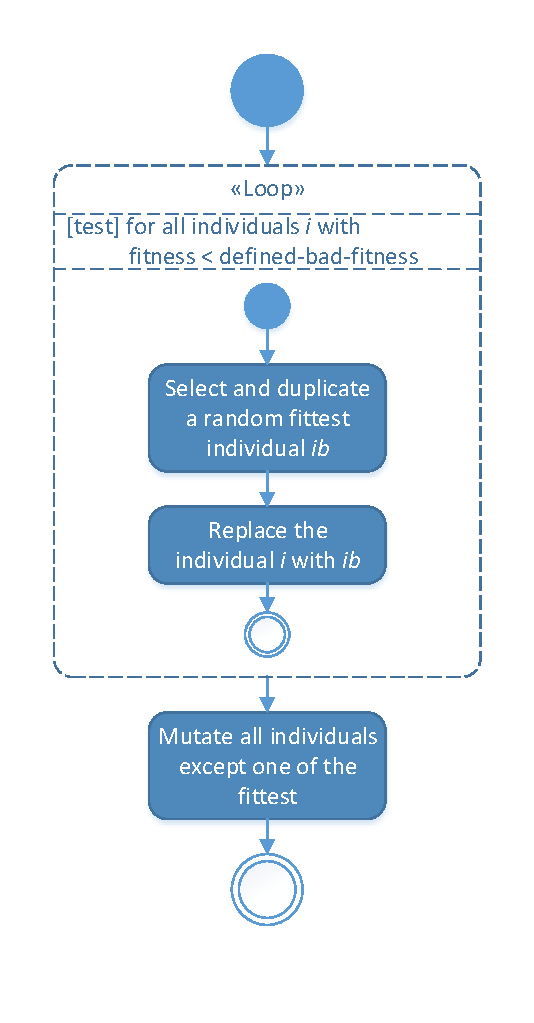
\includegraphics[scale=0.7, trim=0cm 1.5cm 0cm 0.5cm, clip=true]{Images/SelectionAndReplacement_Naive.pdf} 
	\caption{\Gls{SelectionStrategy} and \gls{ReplacementStrategy}: Naive approach with high selection pressure and elitism}
	\label{figSelectionAndReplacement_Naive}
\end{figure}

\textbf{Naive approach with high selection pressure and elitism}: The first approach is presented in figure \ref{figSelectionAndReplacement_Naive} and follows a simple ``high selection pressure" concept. In the strategy all \glspl{Individual} with a bad-fitness, which is defined as 2\%, are replaced by randomly selected duplicates of the fittest. Afterwards, all \glspl{Individual}, except one of the best, are mutated. A best one is kept in order to ensure a monotonically increasing \gls{FitnessFunction} for the \gls{Population}. The strategy exploits and improves currently promising \glspl{CandidateSolution} fast. It also tries to advance all with a fitness between 2\% and 100\%, which are expected to be many. This benefit creates the risk of getting trapped in a \gls{LocalOptimum} and requires a lot of computational power, since almost all \glspl{Individual} are mutated always. % At least 10 \glspl{Individual} are kept in any case, even when all are below 2\% to

\begin{figure}[!ht]
	\centering
	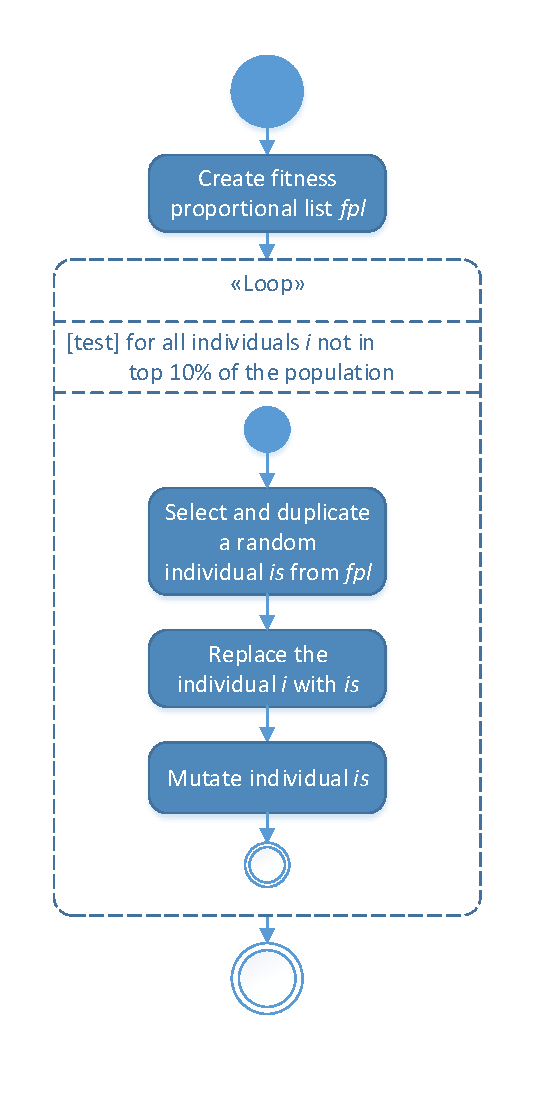
\includegraphics[scale=0.7, trim=0cm 1.5cm 0cm 0.5cm, clip=true]{Images/SelectionAndReplacement_Roulette.pdf} 
	\caption{\Gls{SelectionStrategy} and \gls{ReplacementStrategy}: \Gls{RouletteWheelSelection} with elitism}
	\label{figSelectionAndReplacement_Roulette}
\end{figure}

\textbf{\Gls{RouletteWheelSelection} with elitism}: In order to reduce the change of getting trapped in \gls{LocalOptimum}, the second strategy uses \gls{RouletteWheelSelection} (see sub-section \ref{secEvolutionaryAlgorithms}). Furthermore, instead of using a bad-fitness-constant for the replacement, a fixed fraction of the \glspl{Individual} is used. Since this strategy imposes a greater chance for \glspl{Individual} with bad fitness, it might slow down otherwise.

This strategy creates a fitness proportional list of all \glspl{Individual}. It then replaces all \glspl{Individual} which are not in the top 10\% of the \gls{Population} with duplicates of those (see figure \ref{figSelectionAndReplacement_Roulette}). After the replacement the duplicates are mutated.

\begin{figure}[!ht]
	\centering
	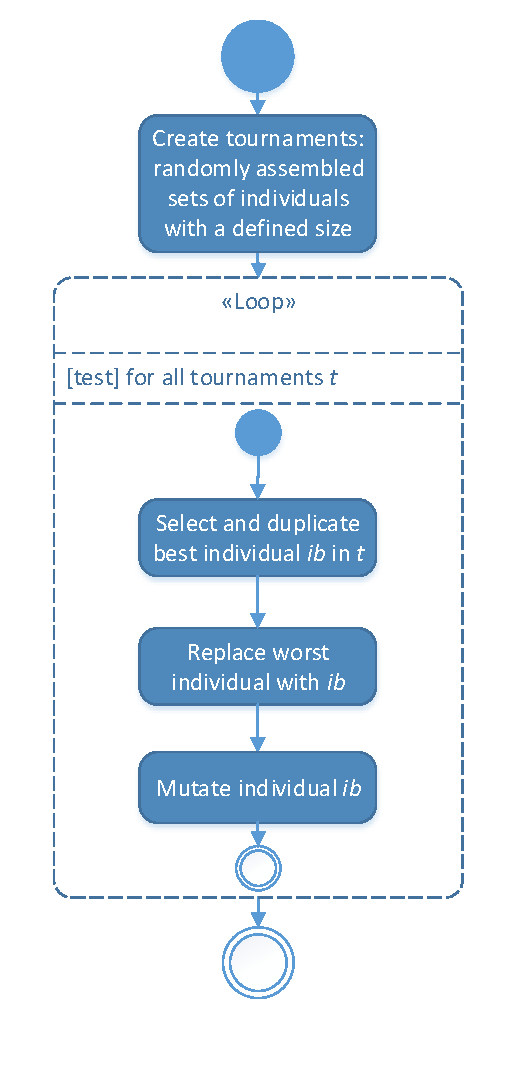
\includegraphics[scale=0.7, trim=0cm 1cm 0cm 0cm, clip=true]{Images/SelectionAndReplacement_Tournament.pdf} 
	\caption{\Gls{SelectionStrategy} and \gls{ReplacementStrategy}: \Gls{TournamentSelection} with elitism}
	\label{figSelectionAndReplacement_Tournament}
\end{figure}

\textbf{\Gls{TournamentSelection} with elitism}: This strategy uses \gls{TournamentSelection} and thus the selection pressure and the required computational power can be fine-tuned by adjusting the tournament size. At first, the tournaments are created with the defined size. A tournament is a randomly assembled proper subset, whereas the intersection of all subsets is empty. Within each the best \gls{Individual} replaces the worst, which is also mutated (see figure \ref{figSelectionAndReplacement_Tournament}). The others remain unchanged. A larger tournament size increases the selection pressure and decreases the required computational power. The strategy is used with a tournament size of two, which is the minimum, and 10.

% use the previously explained \gls{FitnessFunction} and \glspl{Mutation}
%-> ELITISM REQUIRED
%- NaiveMaximumSelectionPressureAlgorithm
%  In the first place instead of sophisticated \glspl{SelectionStrategy}, a naive approach is used which chooses simply all \glspl{Individual} for \gls{Mutation}. This should provide a large \gls{GeneticDiversity} with the risk of not always having a monotonically increasing fitness function.

	%In this phase some \glspl{Individual} are being removed from the \gls{Population}. The naive approach is to remove the ones which have a bad fitness which will be used in the first prototype. However this \gls{Selection} mechanism tends to move the whole \gls{Population} towards \gls{LocalOptimum} and might not find the \gls{GlobalOptimum}. This is because an \gls{Individual} which has a bad fitness in the first place might very well become the optimal solution later after some variations. More sophisticated selection mechanisms are for example the \gls{RouletteWheelSelection} and the \gls{TournamentSelection}. As mentioned before the usage of those advanced methods will depend on the evaluation results. 
	
	%In simple words the whole approach can be described as ``Start with nothing. Try to explore as many directions as possible from there. Follow only the ones that are promising.".
	
%The composition of the next \gls{Generation} is also based on a naive \gls{Elitism} \gls{ReplacementStrategy}. But instead of keeping a fixed number of fittest \glspl{Individual}, a threshold for ``too bad" \glspl{Individual} is being defined. All below are removed and replaced with copies of the fittest. This might limit \gls{GeneticDiversity} and end up in a \gls{LocalOptimum} in general. As the first scenario is simple and the chosen \glspl{SelectionStrategy} should produce a large \gls{GeneticDiversity} in contrast, this should in total result in a fast convergence towards the optimal solution.	

\section{Mutation Selection Strategies}
\label{secMutationSelectionStrategies}

As previously stated, the approach presented in this thesis utilizes many different \glspl{Mutation}, each defining options for a given \gls{ModelToModelTransformation}. A mutation of an \gls{Individual} is the application of a \glspl{Mutation} with a single option. Hence, the option must be selected. This can be performed in two different ways which are described in the following.

%SelectOptionFromAllPossibleDirectly
\textbf{Selection option from all possible}: The first naive strategy selects the option randomly from a list of all possible options. This provides \glspl{Mutation} with a high number of options, a higher chance to be chosen.

%SelectOperatorFirstAndThenAnOption
\textbf{Select operator first and then an option}: This strategy ensures equivalent opportunities for all \glspl{Mutation}, since those are selected randomly at first, followed by a random selection of an option.
